% MSR 2027 -- Technical Papers
% Format: IEEE conference proceedings (24pt title, 10pt text).
% DO NOT use the compsoc / compsocconf options.
% Limit: 10 pages of main text (including figures, tables, and appendices)
%        + 2 pages containing only references.
% Double-anonymous review: do not include names, affiliations, or acknowledgments
% that identify the authors in the submission version.
\documentclass[10pt,conference]{IEEEtran}

\usepackage{cite}
\usepackage{amsmath,amssymb,amsfonts}
\usepackage{algorithmic}
\usepackage{graphicx}
\usepackage{textcomp}
\usepackage{xcolor}
\usepackage{url}

%% \PassOptionsToPackage{hidelinks,unicode}{hyperref} % Example options

%%%%%%%%% PACKAGES

\usepackage{booktabs}     % for nice horizontal lines
%\usepackage{caption}

% --- Preamble (place in your preamble) ---
% \usepackage[switch]{lineno} 
\usepackage{graphicx}
\usepackage{subcaption}
\usepackage{placeins} % for \FloatBarrier to control float placement
\usepackage{float}     % for [H] exact float placement
% Independent "Listing N" float with a two-column (starred) variant for the
% motivating-example diff. newfloat only needs keyval, so it does not pull in
% the caption package (which conflicts with acmart).
\usepackage{newfloat}
\DeclareFloatingEnvironment[name=Listing, fileext=lol, placement=tbp, within=none]{listing}
\usepackage{tcolorbox}
\tcbuselibrary{skins,breakable,listings}
\usepackage{listings}
\usepackage{xcolor}  % table option passed via \PassOptionsToPackage in main.tex
\usepackage{array}
% Listings styles
\lstdefinestyle{code}{
  basicstyle=\ttfamily\small,
  numbers=left, numberstyle=\scriptsize, numbersep=6pt,
  breaklines=true, breakatwhitespace=true,
  frame=single, framerule=0.4pt,
  tabsize=2, showstringspaces=false
}
\lstdefinestyle{cpp}{style=code, language=C++}
\lstdefinestyle{json}{style=code, language=}
\lstdefinestyle{txt}{style=code, language=}

% Ensure circled step numbers in listings render reliably
% Maps Unicode circled digits to the TikZ-based \circled{n} macro
\lstset{literate=
  {❶}{{\circled{1}}}1
  {❷}{{\circled{2}}}1
  {❸}{{\circled{3}}}1
  {❹}{{\circled{4}}}1
  {❺}{{\circled{5}}}1
  {❻}{{\circled{6}}}1
  {❼}{{\circled{7}}}1
}

% A reusable “code card” environment
\newtcblisting{codecard}[2][]{%
  enhanced, breakable,
  colback=white, colframe=black!12,
  boxrule=0.6pt, arc=2mm, left=1mm, right=1mm, top=1mm, bottom=1mm,
  title={#2}, fonttitle=\bfseries\footnotesize,
  listing only, listing options={#1}
}

% --- GitHub-style split-diff support (used in the Motivating Example) ---------
% Per-cell background highlighting via colortbl's \cellcolor (loaded explicitly
% here: the class loads xcolor *without* the table option, so \cellcolor/\rowcolor
% are otherwise undefined). Code is typeset with \lstinline so quotes/brackets
% stay verbatim-safe.
\usepackage{colortbl}
\definecolor{diffadd}{RGB}{225,251,231}   % GitHub-ish light green (added)
\definecolor{diffdel}{RGB}{255,233,232}   % GitHub-ish light red   (removed)
% Minimal Swift language (listings has no built-in Swift definition)
\lstdefinelanguage{Swift}{%
  morekeywords={func,let,var,while,for,in,if,else,guard,return,true,false,nil},
  sensitive=true, morestring=[b]", morecomment=[l]{//}}
% Compact inline style for the diff cells; long UI-locator lines need it small.
\lstdefinestyle{swiftmini}{%
  basicstyle=\ttfamily\scriptsize, columns=fullflexible, keepspaces=true,
  language=Swift, keywordstyle=\bfseries\color{blue!60!black},
  literate={"}{{\textquotedbl}}1}
% +/- gutter glyphs and the gray line-number cell
\newcommand{\gplus}{\textcolor{green!55!black}{\ttfamily\scriptsize +}}
\newcommand{\gminus}{\textcolor{red!70!black}{\ttfamily\scriptsize $-$}}
\newcommand{\dnum}[1]{\textcolor{black!40}{\ttfamily\scriptsize #1}}
% Shorthand: shade the three cells of one diff half-row (color, then lineno/gutter/code)
\newcommand{\dadd}{\cellcolor{diffadd}}
\newcommand{\ddel}{\cellcolor{diffdel}}
% Code cell + keyword: \lstinline cannot be used here because colortbl/array
% re-scans cells and breaks its verbatim catcodes, so we typeset code as plain
% monospace (T1 renders ", [, ], <, > correctly; ~ gives visible indentation).
\newcommand{\cd}[1]{{\ttfamily\scriptsize\strut #1}}
\newcommand{\kw}[1]{\textcolor{blue!60!black}{\textbf{#1}}}
% One full diff line in a single (optionally shaded) cell, so the line number,
% the +/- gutter, and the code share one continuous background. Fixed-width
% \makebox keeps the columns aligned and guarantees the gap after the number.
% #1=row color, #2=line number, #3=gutter glyph (\gplus/\gminus or empty), #4=code
\newcommand{\diffline}[4]{%
  \cellcolor{#1}\makebox[1.3em][r]{\dnum{#2}}\hspace{8pt}%
  \makebox[0.6em][c]{#3}\hspace{6pt}\cd{#4}}



%% \usepackage{soul}
% xcolor is loaded by the class with the 'table' option (now explicitly loaded above)
\usepackage{tabularx}
%% %% Custom packages end here

%% \usepackage{cite}
%% \usepackage{amsmath}
%% \usepackage{booktabs}
\usepackage{wrapfig}
\usepackage{multirow}
\usepackage{multicol}
\usepackage{enumitem}
%% \usepackage{color}
\usepackage{listings}
%% \usepackage{graphicx}
%% \usepackage{rotate}
%% %% \usepackage{url}
%% %\usepackage[hidelinks]{hyperref}
%% \usepackage{breakurl}
%% \usepackage{flushend}
\usepackage{xspace}
%% \usepackage[round-mode=places,round-precision=1,group-separator={,},group-minimum-digits={3},output-decimal-marker={.}, round-pad=false, exponent-mode = threshold, exponent-thresholds = -3:5, tight-spacing=true]{siunitx}
\usepackage{subcaption}
%\usepackage{pgf-pie}
%% \usepackage{bbding}
\usepackage{pifont}
%% \usepackage{seqsplit}
%% \usepackage{pgfplots}
%% \pgfplotsset{width=7cm,compat=1.8}
%% \usepackage{datetime2}

%% % Tikz Figs
\usepackage{tikz}
\tikzset{>=latex}
\usetikzlibrary{shapes.geometric,arrows.meta,positioning,fit,backgrounds,calc} % for flow diagrams and icon pics

%%%%%%%%%
% ---------- Icon pics (line-art, ~0.5 cm) ----------
\tikzset{
  ic/.style={line width=0.6pt, line cap=round, line join=round},
  pics/play/.style={code={
    \draw[ic] (0,0) circle (0.26);
    \fill (-0.08,-0.13) -- (-0.08,0.13) -- (0.16,0) -- cycle;
  }},
  pics/search/.style={code={
    \draw[ic] (0.03,0.06) circle (0.16);
    \draw[ic] (-0.09,-0.06) -- (-0.22,-0.19);
  }},
  pics/bug/.style={code={
    \draw[ic] (0,0) ellipse (0.15 and 0.21);
    \draw[ic] (0,0.21) -- (0,0.30);
    \draw[ic] (0,0.30) circle (0.07);
    \draw[ic] (-0.04,0.36) -- (-0.09,0.43);
    \draw[ic] (0.04,0.36) -- (0.09,0.43);
    \foreach \y in {0.10,0,-0.10}{
      \draw[ic] (-0.13,\y) -- (-0.26,\y+0.05);
      \draw[ic] (0.13,\y) -- (0.26,\y+0.05);
    }
  }},
  pics/shield/.style={code={
    \draw[ic] (0,0.24) -- (-0.17,0.17) -- (-0.17,-0.07)
      .. controls (-0.17,-0.20) and (-0.07,-0.28) .. (0,-0.30)
      .. controls (0.07,-0.28) and (0.17,-0.20) .. (0.17,-0.07)
      -- (0.17,0.17) -- cycle;
    \draw[ic] (-0.08,0.0) -- (-0.02,-0.08) -- (0.10,0.10);
  }},
  pics/funnel/.style={code={
    \draw[ic] (-0.22,0.20) -- (0.22,0.20) -- (0.05,-0.05) -- (0.05,-0.22)
      -- (-0.05,-0.22) -- (-0.05,-0.05) -- cycle;
  }},
  pics/db/.style={code={
    \draw[ic] (-0.16,0.18) arc (180:360:0.16 and 0.07);
    \draw[ic] (-0.16,0.18) arc (180:0:0.16 and 0.07);
    \draw[ic] (-0.16,0.18) -- (-0.16,-0.18);
    \draw[ic] (0.16,0.18) -- (0.16,-0.18);
    \draw[ic] (-0.16,0.0) arc (180:360:0.16 and 0.07);
    \draw[ic] (-0.16,-0.18) arc (180:360:0.16 and 0.07);
  }},
  pics/brain/.style={code={
    \draw[ic] (0,0.26)
      .. controls (-0.22,0.26) and (-0.28,0.08) .. (-0.20,-0.02)
      .. controls (-0.30,-0.10) and (-0.20,-0.28) .. (-0.05,-0.22)
      .. controls (0.0,-0.30) and (0.0,-0.30) .. (0.05,-0.22)
      .. controls (0.20,-0.28) and (0.30,-0.10) .. (0.20,-0.02)
      .. controls (0.28,0.08) and (0.22,0.26) .. (0,0.26) -- cycle;
    \draw[ic] (0,0.26) -- (0,-0.24);
    \draw[ic] (-0.10,0.12) .. controls (-0.02,0.10) and (-0.02,0.0) .. (-0.10,-0.04);
    \draw[ic] (0.10,0.12) .. controls (0.02,0.10) and (0.02,0.0) .. (0.10,-0.04);
  }},
  pics/book/.style={code={
    \draw[ic] (0,-0.16) .. controls (-0.10,-0.24) and (-0.24,-0.20) .. (-0.26,-0.16)
      -- (-0.26,0.16) .. controls (-0.20,0.12) and (-0.06,0.10) .. (0,0.18);
    \draw[ic] (0,-0.16) .. controls (0.10,-0.24) and (0.24,-0.20) .. (0.26,-0.16)
      -- (0.26,0.16) .. controls (0.20,0.12) and (0.06,0.10) .. (0,0.18);
    \draw[ic] (0,0.18) -- (0,-0.16);
  }},
  pics/graph/.style={code={
    \draw[ic] (-0.30,0) -- (0.30,0);
    \draw[ic] (0,0) -- (0,0.20);
    \foreach \x in {-0.30,-0.10,0.10,0.30}{ \fill (\x,0) circle (0.035); \draw[ic] (\x,0) circle (0.035);}
    \fill (0,0.20) circle (0.035); \draw[ic] (0,0.20) circle (0.035);
  }},
  pics/repo/.style={code={
    \draw[ic] (-0.10,0.26) -- (-0.10,-0.26);
    \foreach \y in {0.20,-0.04,-0.20}{ \fill (-0.10,\y) circle (0.05); \draw[ic](-0.10,\y) circle (0.05);}
    \draw[ic] (-0.10,-0.04) .. controls (0.06,-0.04) and (0.16,0.04) .. (0.16,0.16);
    \fill (0.16,0.20) circle (0.05); \draw[ic] (0.16,0.20) circle (0.05);
  }},
}
%%%%%%%%%


%% %\usepackage{pgf-umlsd} % for flow diagram
%% \usetikzlibrary{calc}
%% \usetikzlibrary{shapes.geometric}
%% \usetikzlibrary{decorations.pathreplacing}
%% \usetikzlibrary{positioning}
\newcommand*\circled[1]{\tikz[baseline=(char.base)]{
            \node[shape=circle,draw,fill=black,text=white,inner
            sep=0.4pt] (char) {\small #1};}}

%% %%%%%%%%%% CHECKMARKS


%% %%%%%%%% CONCLUDING BOXES
\usepackage[framemethod=tikz]{mdframed}
\mdfdefinestyle{mpdframe}{
   frametitlebackgroundcolor   =black!15,
    frametitlerule              =true,
    roundcorner                 =3pt,
    middlelinewidth             =1pt,
    skipabove                   =\topskip,
    skipbelow                   =\topskip,
    innermargin                 =0.1cm, % smaller makes box bigger
    outermargin                 =0.1cm,
    innerleftmargin             =0.1cm,
    innerrightmargin            =0cm,
    innertopmargin              =0.1cm,
    innerbottommargin           =0.1cm,
    align=center   
}

%%%%%%%%%% CODE and MACROS

%\input{defs-code}
%% \input{defs-logic}

%%%%%%%%%% UNCLASSIFIED
\newcommand{\Caption}[1]{\caption{#1}}
\newcommand{\NAtname}{-}
\newcommand{\specialcell}[2][c]{\begin{tabular}[#1]{@{}c@{}}#2\end{tabular}}
% Right-aligned special cell for numbers with inline deltas
\newcommand{\specialcellr}[1]{\begin{tabular}[c]{@{}r@{}}#1\end{tabular}}
\newcommand{\DefMacro}[2]{%
   \expandafter\newcommand\csname rmk-#1\endcsname{#2}%
}
\newcommand{\UseMacro}[1]{\csname rmk-#1\endcsname}


\newcommand{\YC}{\textcolor{blue}{\textbf{+}}} %{$\checkmark$}}
\newcommand{\NC}{\textcolor{red}{\textbf{-}}} %\textbf{$\times$}}}
\newcommand{\MC}{\textcolor{magenta}{\textbf{$\pm$}}}

\newcommand{\etal}{et al.}
\newcommand{\eg}{e.g.}
\newcommand{\ie}{i.e.}
\newcommand{\Fix}[1]{\textcolor{red}{[#1]}}
\newcommand{\Fixsd}[1]{\textcolor{purple}{SD:[#1]}}
\newcommand{\Bren}[1]{\textcolor{teal}{Breno:~[#1]}}
\newcommand{\Den}[1]{\textcolor{blue}{Denini:~[#1]}}


\newcommand{\TODO}[1]{{\color{red}{\bf TODO:} #1}}
\newcommand{\Comment}[1]{}
\newcommand{\Boldface}[1]{\textbf{#1}}
\newcommand{\Space}[1]{}
\newcommand{\hand}[1]{\textcolor{green}{[#1]}}
\newcommand{\raw}[1]{\textcolor{red}{#1}}
\newcommand{\edit}[1]{#1}

\newcommand{\MeanStd}[2]{#1$\pm$#2}
\newcommand{\MeanStdSec}[2]{#1$\pm$#2 seconds}
\newcommand{\plus}{$+$}

\newcommand{\MyPara}[1]{\vspace{1pt}\noindent\textbf{#1}.}
\newcommand{\MyParaOnly}[1]{\noindent\textbf{#1}}
\newcommand{\MyItPara}[1]{\noindent\textit{#1}.}
\newcommand{\reducedstrut}{\vrule width 0pt height .9\ht\strutbox depth .9\dp\strutbox\relax}
%\newcommand{\InputWithSpace}[1]{\bgroup\def\arraystretch{1.1}\input{#1}\egroup}
\newcommand{\Code}[1]{{\small\ifmmode{\texttt{#1}}\else$\texttt{#1}$\fi}}
\newcommand{\CodeIn}[1]{{\small\ifmmode{\mathtt{#1}}\else$\mathtt{#1}$\fi}}
\newcommand{\ColorBack}[1]{%
  \begingroup \setlength{\fboxsep}{0pt}% \colorbox{purple!20}{\reducedstrut#1\/}% \endgroup
}

%% % ----------
%% % THIS BELOW COPIED FROM vkuncak/doc/vmcai09/defs.tex
\definecolor{gray}{RGB}{211,211,211}



% Define the TODO command with highlight and margin note
\newcommand{\todo}[2][normal]{%
  \ifdefined\showtodos
    \ifstrequal{#1}{high}{\sethlcolor{red}}{}%
    \ifstrequal{#1}{normal}{\sethlcolor{yellow}}{}%
    \ifstrequal{#1}{low}{\sethlcolor{green}}{}%
    {\hl{\textbf{TODO:} #2}}%
    \marginpar{\textcolor{red}{\textbf{TODO}}}%
  \fi
}

% Control visibility of TODOs with this toggle
\newif\ifshowtodos
\showtodostrue  % Set to \showtodosfalse before final submission



%%%%%%

%%
%% end of the preamble, start of the body of the document source.
\setkeys{Gin}{draft=false}
\renewcommand{\lstlistingname}{Listing}
\usepackage{tcolorbox}
\usepackage{multirow}
\usepackage{placeins}
\usepackage[hidelinks]{hyperref}
\usepackage{makecell}
\usepackage{tabularx}
\usepackage{array}
\usepackage{fvextra}
\usepackage{microtype}
\emergencystretch=2em
\raggedbottom

\newenvironment{packed_itemize}{
\vspace{-0.1ex}
\begin{list}{\labelitemi}{\leftmargin=1.7em}
 \setlength{\itemsep}{0pt} \setlength{\parskip}{0pt} \setlength{\parsep}{0pt} \setlength{\headsep}{0pt} \setlength{\topskip}{0pt} \setlength{\topmargin}{0pt} \setlength{\topsep}{0pt} \setlength{\partopsep}{0pt}
 }{\end{list}
\vspace{-0.1ex}
}


\newcommand{\tool}{\texttt{FLAG}}
\newcommand{\pcount}{\textsc{2}}
\newcommand{\x}{x\xspace}
\newcommand{\Contrib}[1]{$\star$#1}
\newcommand{\sota}{SoTA\xspace}

\newcommand{\repository}{https://github.com}

\usepackage{pifont}% http://ctan.org/pkg/pifont
\newcommand{\cmark}{\ding{51}}%
\newcommand{\xmark}{\ding{55}}%

\definecolor{codebg}{rgb}{0.95, 0.95, 0.92} % Light background
\definecolor{keywordcolor}{rgb}{0.0, 0.0, 0.6} % Blue for keywords
\definecolor{stringcolor}{rgb}{0.58, 0.0, 0.82} % Purple for strings
\definecolor{commentcolor}{rgb}{0.0, 0.5, 0.0} % Green for comments 

\lstset{
    language=Go,              % Language
    backgroundcolor=\color{codebg}, % Background color
    basicstyle=\ttfamily\small, % Font type and size
    keywordstyle=\color{keywordcolor}\bfseries, % Style for keywords
    stringstyle=\color{stringcolor}, % Style for strings
    commentstyle=\color{commentcolor}\itshape, % Style for comments
    numbers=left,               % Line numbers on the left
    numberstyle=\tiny,          % Line number font size
    stepnumber=1,               % Line numbering step
    frame=single,               % Frame around the code
    breaklines=true,            % Line breaking
    tabsize=2,                  % Tab size
    showspaces=false,           % Don't display spaces
    showstringspaces=false,     % Don't display string spaces
    captionpos=b,               % Caption position (b for bottom)
    lineskip=1pt,
    linewidth=1\columnwidth,
    xleftmargin=13pt,    % Add padding to the left
    numbersep=5pt,
    escapeinside={(*@}{@*)}, % Allows inline LaTeX
}


\newcommand{\myparagraph}[1]{\vspace{0.5ex}\noindent \textbf{#1. }}

%% Placeholder for numbers that depend on experiments not yet run.
%% Grep for \PENDING before submitting -- none must remain.
\newcommand{\PENDING}[1]{\textcolor{red}{\textbf{[PENDING: #1]}}}


\begin{document}

\title{The Vocabulary of Flaky Tests in C\#}

% Anonymous submission (double-anonymous). Restore the authors only in the camera-ready version.
\author{\IEEEauthorblockN{Anonymous Author(s)}
\IEEEauthorblockA{\textit{Omitted for double-anonymous review}}
}

\maketitle

\begin{abstract}
Flaky tests produce non-deterministic outcomes on an unchanged codebase, eroding trust in continuous integration. Vocabulary-based prediction reports high scores for Java, JavaScript, and Swift, although replications show that performance drops under more realistic evaluation. To the best of our knowledge, it has never been evaluated for C\#, whose concurrency model (\texttt{Task}, \texttt{async}/\texttt{await}) and testing frameworks differ from those previously studied. We re-ran the test suites of 17 open-source C\# projects, totaling 19,211 test cases, 100 times, and up to 20 more times in isolation. After grouping by declaring method, we obtained 30 flaky and 12,635 stable test methods, and we trained eight classifiers on TF-IDF features of unigrams and bigrams. The best ones, Extra Trees and Random Forest, reach an MCC of 0.51--0.53 and an AUC of 0.86--0.87 in cross-validation, only moderately above a vocabulary-threshold rule (MCC 0.40) and a structure-only model (MCC 0.36). With the labels of the 20-run round, the structure-only model catches up with them. On repositories left out of training, AUC drops to 0.75--0.78 and precision to 2--3\%, yet the top quartile of each repository's ranking still contains 23 of the 30 flaky tests. Vocabulary can therefore prioritize reruns, but it cannot gate pipelines. The markers of flakiness are Task-based concurrency, time handling, and resource lifecycles, and no robust marker of stability emerges. The model fails when the root cause lies outside the test body or when asynchronous constructs are used deterministically, which exposes the limited reach of vocabulary. \Den{Sugestão de título: ``Does Flaky-Test Vocabulary Carry Over to C\#?''}
\end{abstract}

\begin{IEEEkeywords}
flaky tests, test flakiness, software testing, vocabulary-based prediction, C\#, .NET
\end{IEEEkeywords}

\section{Introduction}
\label{sec:intro}
In software development, tests are essential for identifying defects and verifying that fixes work correctly \cite{kapfhammer2004software}. Ideally, test results remain stable across runs of an unchanged codebase. However, flaky tests, that is, tests that pass or fail nondeterministically on the same version of the code, are a common reality \cite{parry2021survey, pinto2020vocabulary}. Their causes are diverse, including concurrency issues, asynchronous operations, order dependencies between tests, improper management of external resources, dependence on the system clock, and the use of random values \cite{luo2014empirical}, as well as overly narrow ranges of expected values and timeout-related issues \cite{eck2019understanding}.

Although flaky tests do not directly affect software functionality, they impose a substantial cost on delivery pipelines. Developers report wasted effort analyzing failures, ignored failures, and loss of trust in the test suite \cite{eck2019understanding, gruber2022survey}, and at Google about 16\% of tests show some level of flakiness, with 2\% to 16\% of compute resources spent on rerunning them \cite{micco2017state}. Detecting flakiness through reruns is expensive, since tests that fail rarely require many executions \cite{lam2020study}. Static prediction from the test code is therefore attractive: it requires running nothing, and its features can be inspected by developers.

Pinto et al.~\cite{pinto2020vocabulary} showed that flaky tests share a characteristic vocabulary, that is, identifiers and keywords that occur disproportionately in them, and achieved an F-score of 0.95 in Java. The idea was replicated for Java with more classifiers and an inter-project evaluation \cite{camara2021revisiting}, for Python \cite{haben2021replication}, JavaScript \cite{soratto2023vocabulary}, and Swift \cite{medeiros2026vocabulary}, and extended to five languages \cite{ahmad2025understanding}. These studies also expose its limits. Performance drops sharply across projects \cite{camara2021revisiting, soratto2023vocabulary} and over time \cite{haben2021replication}, the predictions were not actionable in an industrial setting \cite{berndt2023vocabulary}, and code-based detectors do not beat a majority baseline once projects are kept apart \cite{gultekin2026limits}.

To the best of our knowledge, vocabulary-based prediction has never been evaluated for C\#, even though flakiness in .NET projects is well documented \cite{lam2019root, lam2020study, leesatapornwongsa2022flakerepro} and the language has relevant particularities. Its concurrency model centers on the Task-based asynchronous pattern (\texttt{Task}, \texttt{async}/\texttt{await}, \texttt{CancellationToken}) and the thread pool, which introduces its own timing and scheduling dependencies. In tests from Microsoft .NET projects, concurrency is the leading cause of flakiness, with fixed waits and timeouts as a frequent pattern \cite{leesatapornwongsa2022flakerepro}. Test suites are written with several testing frameworks (xUnit, NUnit, and MSTest) and run on two test platforms (VSTest and the newer Microsoft.Testing.Platform), and libraries are often compiled for multiple target frameworks, so the same test may run under different runtimes. \Den{Nenhum dos 17 projetos usa MSTest (Seção~\ref{sec:subjects}), e as particularidades deste parágrafo (frameworks, multi-target, locale/time zone, containers) não são analisadas depois. Ou se faz uma análise por framework/TFM (os tokens e o desempenho mudam entre xUnit e NUnit?), ou se enxuga o parágrafo para não prometer o que o artigo não entrega.} Integration suites also depend on containerized services and on environment behaviors such as locale, time zone, and file system paths. If the lexical patterns that signal flakiness in Java, JavaScript, and Swift do not transfer to C\#, vocabulary-based tools built around them would offer little help to .NET developers. This is the gap this work addresses. \Den{A lacuna é formulada como ``os padrões transferem para C\#?'', mas nenhuma RQ testa transferência. Sugestão de RQ nova: comparar sistematicamente o vocabulário de C\# com as listas publicadas para Java (Pinto), JS (Soratto), Swift (Medeiros) e Python (Haben), por exemplo pela sobreposição dos top-$k$ tokens após normalização (sleep, thread, wait, async, timeout...). Uma versão mais forte: treinar com dados de outra linguagem e testar em C\#. Isso também justificaria o título.}

To address it, we investigate static prediction of flaky tests in C\# from the vocabulary of test source code. Our approach, organized in six steps (Section~\ref{sec:approach}), selects open-source C\# projects and systematically reruns their test suites, 100 times in an automated fashion and again 20 times under controlled isolation; labels each test as flaky, broken, or stable according to its outcomes; resolves inherited tests to the method that declares them; extracts the vocabulary and structural features of each test with the Roslyn compiler platform; and trains classifiers on this vocabulary to predict a test's propensity to be flaky without executing it, while also extracting an interpretable ranking of the tokens most strongly associated with flakiness. We ask the following research questions:

\begin{description}[leftmargin=1.2em,labelindent=0pt,itemsep=1pt]
  \item[RQ1.1] How accurately can flaky tests in C\# be predicted from the vocabulary of their source code?
  \item[RQ1.2] Do the labels and results remain stable between the 100-run and the 20-run rounds?
  \item[RQ2] Does vocabulary-based prediction outperform the majority, random, vocabulary-threshold, and structure-only baselines?
  \item[RQ3] Which tokens are most strongly associated with flakiness?
  \item[RQ4] When and why does the classifier fail?
\end{description}

We applied this methodology to 17 projects, with 19,211 test cases and 12,665 labeled test methods, of which 30 are flaky and 12,635 are stable (0.24\%). Among the eight classifiers evaluated, tree ensembles performed best under cross-validation, with Extra Trees reaching an MCC of 0.53 and an AUC of 0.86, and Random Forest an MCC of 0.51 and an AUC of 0.87. These results are well above random guessing (MCC 0.02), but only moderately above a structure-only baseline (MCC 0.36) and a vocabulary threshold rule (MCC 0.40) (RQ1.1, RQ2). With the labels of the 20-run round, the structure-only model catches up with the ensembles, so the advantage of vocabulary depends on the round that produced the labels (RQ1.2). When each repository is held out and evaluated at its natural base rate, AUC drops to 0.75--0.78 and precision stays at 2--3\%. The approach is therefore better suited to ranking tests and prioritizing reruns than to gating a pipeline, since the top quartile of each repository's ranking contains 23 of the 30 flaky tests. The signal rests on Task-based concurrency, time handling, and resource lifecycles (RQ3), and the model fails when the cause lies outside the test body or when asynchronous constructs are used deterministically (RQ4).

The main contributions of this work are:
\begin{packed_itemize}
  \item[$\star$] A dataset of flaky, broken, and stable C\# tests, built from 100 automated and 20 controlled reruns of 17 open-source projects, with inherited tests resolved to the methods that declare them.
  \item[$\star$] An evaluation of eight classifiers for vocabulary-based static prediction in C\#, under repeated cross-validation and under cross-repository validation at the natural base rate, showing that a lexical signal exists in C\# but is modest under realistic evaluation.
  \item[$\star$] A C\# flakiness vocabulary, which separates frequent general markers from rare, specific ones and shows that no robust marker of stability emerges.
  \item[$\star$] An analysis of the model's errors in the test code, with sensitivity analyses without attributes and with helper-method expansion, which outline the limits of lexical prediction.
  \item[$\star$] An assessment of label robustness, comparing the two rerun rounds (which agree on only 13 of the 36 flaky tests), and documentation of the pitfalls of rerun studies in .NET that distorted our initial counts (Table~\ref{tab:armadilhas}).
\end{packed_itemize}
\Den{Posicionamento para o ISSTA: replicar o método numa linguagem nova tende a ser visto como incremental (perfil mais de MSR/ESEM/SAST). As contribuições mais originais aqui são (i) o protocolo e as armadilhas de reruns em .NET, (ii) a sensibilidade dos rótulos à rodada e (iii) a avaliação realista (LOPO, taxa natural, ranking). Sugiro organizar a narrativa em torno disso e deixar ``vocabulário em C\#'' como veículo. A última contribuição enquadra a sobreposição 13/36 como ``robustez''; ver o comentário na RQ1.2.}


\section{Motivating Example}
\label{sec:motivation}

Consider \texttt{ReconnectOnRouterBug}, a test from NetMQ, a messaging library in the .NET ecosystem, which was flaky in our 100-run round. The test checks a reconnection behavior. It connects a router socket to a dealer, sends a message, disconnects, reconnects, and sends the message again. The goal is to ensure that the second message also reaches its destination after reconnection (abbreviated in Listing~\ref{lst:flaky}). \Den{Informar quantas vezes este teste falhou nas 100 execuções (k/100).}

\begin{listing}[!htbp]
\begin{lstlisting}[language={[Sharp]C}, basicstyle=\ttfamily\footnotesize, columns=fullflexible, keepspaces=true, backgroundcolor={}, frame=tb, framerule=0.4pt, numberstyle=\tiny\color{black!45}, numbersep=4pt, xleftmargin=1em, framexleftmargin=1em, breaklines=false, emph={Sleep}, emphstyle={\color{red!70!black}\bfseries}]
router.Connect(addr);
Thread.Sleep(100);
router.SendMoreFrame("dealer").SendFrame("Hello");
router.Disconnect(addr);
Thread.Sleep(1000);
router.Connect(addr);
Thread.Sleep(100);
router.SendMoreFrame("dealer").SendFrame("Hello");
\end{lstlisting}
\caption{Flaky test with fixed waits (abbreviated).}
\label{lst:flaky}
\end{listing}

The key point is that the test has no mechanism for synchronizing with what happens inside the library. Connecting and disconnecting a socket are asynchronous operations: the \texttt{Connect} call returns before the connection is actually established. The test works around this with fixed waits (\texttt{Thread.Sleep(100)} after each connection and \texttt{Thread.Sleep(1000)} after disconnection). Each of these waits is a bet on how long the connection takes. If the bet holds in most runs, the test passes. But in a slower or more heavily loaded run, such as on a shared continuous integration machine, the connection may take longer than the wait. The second send then reaches the socket before the reconnection is reestablished, and the test fails, without anything in the code having changed.

This kind of failure is expensive to expose by plain reruns. It depends on a sub-second time window and on load conditions we do not control, and therefore it does not reproduce on demand. Confirming that the test is flaky required repeating the suite 100 times, and a smaller sample might not have observed the failure. Indeed, the test did not fail in our second round of 20 runs (Section~\ref{sec:rq12}). The situation is that of a developer who sees the test fail once in continuous integration, reruns it, sees it pass, and dismisses the failure as noise. This cycle is the wasted effort and loss of trust described in Section~\ref{sec:intro}.

Even so, the likely cause is visible in the source code. The test is dominated by socket calls (\texttt{Connect}, \texttt{Disconnect}, \texttt{SendFrame}) interleaved with \texttt{Thread.Sleep}, and it contains no wait for an event, such as confirmation that the connection has been established. This is the starting point of our work: a failure that manifests only at run time can leave a lexical trace in the test's text. If this trace exists and is consistent, a model trained only on the code's terms can point to the most suspicious tests without running them. Section~\ref{sec:rq4} returns to this test for a complementary reason: the model ranked it low. The trace here is a synchronous \texttt{Sleep}, not the \texttt{async}/\texttt{await} vocabulary that dominates the flaky tests in our dataset, which suggests that the model recognizes one kind of cause better than another. \Den{O exemplo motivador é um caso que o modelo \emph{erra} (ranqueado baixo). Isso enfraquece a motivação: o leitor termina a seção achando que a abordagem não funciona justamente no caso apresentado. Sugiro usar como exemplo motivador um flaky bem ranqueado (com \texttt{Task.Delay}/\texttt{CancellationToken}) e manter o \texttt{ReconnectOnRouterBug} na RQ4 como falso negativo.}


\section{Related Work}
\label{sec:related}

\myparagraph{Flaky tests} A flaky test produces different outcomes across runs of the same software version \cite{luo2014empirical, parry2021survey}. Developers spend considerable effort triaging failures that do not signal a real defect \cite{pinto2020vocabulary}, and repeated exposure erodes trust to the point that genuine failures are ignored \cite{gruber2022survey, rahman2018impact}; the cost to delivery pipelines is also documented \cite{herzig2015empirically, micco2017state}.

\myparagraph{Detection} Techniques are dynamic, hybrid, or static, depending on whether they require running the test. Rerunning the suite is practiced at scale at Google and Microsoft \cite{lam2020study, micco2017state}, but its cost grows with the rerun budget, and even five reruns reveal only about 88\% of flaky tests \cite{lam2020understanding}. \Den{Conferir este número na fonte (Lam et al., ISSRE 2020).} iDFlakies reruns suites in different orders to separate order-dependent tests from the others \cite{lam2019idflakies}. DeFlaker flags tests that fail without exercising modified code \cite{bell2018deflaker}; Shaker injects stress to expose concurrency-related flakiness \cite{silva2020shake}. Several tools target .NET directly. RootFinder analyzes logs of passing and failing runs to root-cause flaky tests at Microsoft \cite{lam2019root}, TSVD detects thread-safety violations in C\# code during testing \cite{li2019tsvd}, and FlakeRepro \cite{leesatapornwongsa2022flakerepro} combines static and dynamic analysis to reproduce the failure of a concurrency-related flaky test: across 31 flaky tests from 22 Microsoft projects, it reproduced 26. FlakeSync repairs flaky tests caused by asynchronous waits \cite{rahman2024flakesync}. These tools require the test binaries and, in most cases, an observed failure, so they act during debugging after flakiness has been found, whereas our approach predicts which tests are likely flaky from source code alone and can feed into them.

\myparagraph{Vocabulary-based prediction} Pinto et al.~\cite{pinto2020vocabulary} trained classifiers on the vocabulary of test code (F1 = 0.95 in Java). Camara et al.~\cite{camara2021revisiting} replicated the study with more classifiers and found that recall falls to about 0.02 in an inter-project evaluation; Haben et al.~\cite{haben2021replication} carried it to Python and observed that a time-based split lowers performance; and Soratto and Silva~\cite{soratto2023vocabulary} reported a cross-project F1 of 0.07 for JavaScript. Ahmad et al.~\cite{ahmad2025understanding} compared five languages, and Medeiros et al.~\cite{medeiros2026vocabulary} studied Swift and found a vocabulary of asynchronous constructs and stability markers. In an industrial setting, Berndt et al.~\cite{berndt2023vocabulary} found that the predictions, despite high F-measures, were not actionable for developers. Other static predictors reach similar conclusions: FlakeFlagger \cite{alshammari2021flakeflagger} reports that tokens of the test source were not effective predictors and relies on behavioral features such as coverage and execution time, FLAST \cite{verdecchia2021know} classifies tests by similarity to known flaky ones, and Pontillo et al.~\cite{pontillo2022static} and Gruber et al.~\cite{gruber2023practical} evaluate static and history-based features under more realistic conditions. Barbosa et al.~\cite{barbosa2023test} show that root causes vary by ecosystem. \Den{Verificar se C\# está entre as linguagens estudadas por Barbosa et al.; se estiver, citar os resultados para C\# e ajustar a afirmação de novidade.} Table~\ref{tab:literatura} summarizes the published intra-project results. They are consistently high, whereas cross-project results are consistently low. No vocabulary-based study covers C\#.

\begin{table}[!htbp]
\caption{Published intra-project results for vocabulary-based flaky-test prediction. N: tests in the evaluated dataset.}
\label{tab:literatura}
\centering
\footnotesize
\setlength{\tabcolsep}{3pt}
\begin{tabular}{@{}llrcccl@{}}
\toprule
\textbf{Study} & \textbf{Lang.} & \textbf{N} & \textbf{P} & \textbf{R} & \textbf{F1} & \textbf{Protocol} \\
\midrule
Pinto et al.~\cite{pinto2020vocabulary} & Java & 2,806 & 0.99 & 0.91 & 0.95 & 80/20 \\
Camara et al.~\cite{camara2021revisiting} & Java & 2,806 & 0.98 & 0.89 & 0.94 & 80/20 \\
Haben et al.~\cite{haben2021replication} & Python & 20,641 & 0.94 & 0.74 & 0.80 & 80/20 \\
Soratto and Silva~\cite{soratto2023vocabulary} & JS & 868 & --- & 0.72 & 0.82 & 80/20 \\
Medeiros et al.~\cite{medeiros2026vocabulary} & Swift & 182 & 0.92 & 0.83 & 0.87 & $k$-fold \\
\midrule
This work (Extra Trees) & C\# & 60$^{a}$ & 0.87 & 0.63 & 0.69 & 5-fold $\times$ 10 \\
\bottomrule
\end{tabular}

\vspace{0.2em}
\raggedright\footnotesize $^{a}$30 flaky and 30 stable tests per undersampling draw, out of 12,665 labeled methods.
\end{table}

\myparagraph{Positioning} Cross-project evaluation is not new \cite{camara2021revisiting, soratto2023vocabulary, gultekin2026limits}, and we adopt it rather than claim it. This work differs from previous ones in three respects. First, we document the pitfalls of rerun studies in .NET (Table~\ref{tab:armadilhas}) and use the declaring method, with inheritance resolved, as the unit of analysis instead of the test case. Second, we compare two rerun rounds and measure how much the labels, and the conclusions drawn from them, depend on the round. Third, we evaluate the ranking produced by the model at the natural rate of flaky tests, with average precision and the share of flaky tests found in the top of each repository's ranking, and we separate frequent, general markers from rare, specific ones instead of treating the vocabulary as a single ranking. \Den{Se o paper de Go estiver publicado (ou no arXiv) antes da submissão, citá-lo em terceira pessoa (atenção ao double-blind) e alinhar as conclusões: lá o nome do repositório empata com o vocabulário, e um revisor que conheça os dois vai cobrar o mesmo baseline aqui.}

\myparagraph{Learned features} Pre-trained models such as CodeBERT \cite{fatima2022flakify} and prompting-based use of LLMs \cite{berndt2026can} provide mixed evidence: learned features help more in categorizing root causes than in binary prediction \cite{rahman2024quantizing}, accuracy drops considerably under realistic imbalance \cite{rahman2025understanding}, and code-based detectors lose most of their advantage once the evaluation separates projects \cite{gultekin2026limits}. Vocabulary features remain cheap and interpretable. \Den{Em 2027 os revisores vão pedir ao menos um baseline de modelo pré-treinado (Flakify/CodeBERT) ou de LLM com prompt (como Berndt et al. 2026 e a RQ4 do paper de Go). Com 30 positivos o fine-tuning é inviável, mas um LLM zero-shot sobre os 30 flaky e uma amostra de estáveis é barato e responde à pergunta ``por que não LLM?''.}


\section{Approach}
\label{sec:approach}
Our approach rests on one premise: although flakiness manifests only at run time, it leaves a stable lexical trace in the test code. Figure~\ref{fig:metodologia} summarizes the six-step pipeline.

\begin{figure*}[!htbp]
\centering
{\scriptsize
\setlength{\fboxsep}{3pt}%
\newcommand{\etapa}[2]{\fbox{\parbox[c][13.5ex][c]{\dimexpr(\textwidth-55pt)/6-2\fboxsep-2\fboxrule\relax}{\centering\hyphenpenalty=10000\textbf{#1}\\[2pt]#2}}}%
\etapa{1. Subjects}{17 open-source\\C\# projects;\\19,211 test cases}%
\hfill$\rightarrow$\hfill
\etapa{2. Reruns}{100$\times$ + 20$\times$\\isolated;\\TRX reports}%
\hfill$\rightarrow$\hfill
\etapa{3. Labels}{flaky, broken,\\stable, skipped;\\12,665 methods,\\30 flaky}%
\hfill$\rightarrow$\hfill
\etapa{4. Processing}{Roslyn: tokens\\and structure}%
\hfill$\rightarrow$\hfill
\etapa{5. Models}{TF-IDF;\\8 classifiers;\\1:1; CV and LOPO}%
\hfill$\rightarrow$\hfill
\etapa{6. Vocabulary}{information\\gain of\\tokens}%
}
\caption{End-to-end pipeline for building the vocabulary of flaky tests in C\#.}
\label{fig:metodologia}
\end{figure*}

\myparagraph{Step 1: Project selection} We started from open-source C\# libraries hosted on GitHub with extensive test suites and then filtered them by an objective criterion: the project had to build and run its entire suite in our environment. \Den{Do jeito que está, a seleção não é reproduzível. Faltam: como os candidatos foram encontrados (busca no GitHub? lista curada?), quais critérios (estrelas, atividade, número de testes), quantos candidatos foram tentados e quantos falharam no filtro, e em qual commit (SHA) cada projeto foi analisado. O filtro ``builda e roda tudo'' gera viés de sobrevivência para suítes fáceis de executar.} The result is 17 projects and 19,211 test cases, covering messaging, actor systems, scheduling, RPC, logging, resilience, and architecture testing. Two candidate projects (StackExchange.Redis and SSH.NET) were excluded because their suites depend on external servers whose runs were disrupted by the environment.

\myparagraph{Step 2: Reruns} Each suite was built once and run 100 times in a row, without rebuilding between runs. \Den{A ordem dos testes é a mesma em todas as execuções? Se for, a flakiness dependente de ordem (OD) não é exposta e o estudo cobre essencialmente NOD; dizer isso explicitamente, como Pinto et al. Informar também a configuração de paralelismo (o xUnit paraleliza coleções por padrão, o NUnit não), os timeouts e o que acontece quando o runner trava.} In each run, the .NET test runner (\texttt{dotnet test}) produced a TRX (Test Results XML) report, an XML file recording each executed test. We built with \texttt{dotnet build} and ran with \texttt{dotnet test --no-build} and the TRX logger; xUnit v3 projects on Microsoft.Testing.Platform were run through the test executable itself, with \texttt{--report-trx}. These reports were the basis for identifying tests whose outcomes changed across runs. Some rounds suffered environmental disruptions, such as leftover containers from previous runs and a degraded Redis cluster. They were discarded and repeated in isolation. Since flakiness is rare (fewer than 1\% of tests), a few unstable tests are enough to change the results, and any environmental noise could be mistaken for flakiness. We therefore performed a second round of 20 runs under controlled isolation (5 for Testcontainers, whose suite requires containers) to check the tests flagged in the first and to look for flaky tests that the first round missed. Since a single pass/fail flip on the same version already shows that a test is flaky, the second round can add flaky tests but cannot refute those found in the first; Section~\ref{sec:rq12} compares the two rounds. Everything ran on a laptop with an Intel Core i7-1165G7, 16 GB of RAM, and Windows 11. \Den{Sugestão (requer execução): uma rodada adicional em CI (GitHub Actions/Linux) ou com stress de CPU (estilo Shaker) aumentaria o número de positivos e responderia à crítica sobre máquina única. A limitação já foi registrada nas ameaças (Seção~\ref{sec:threats}).} The 100-run rounds took place in July 2026, before a .NET SDK update whose previous version we did not record; the 20-run rounds used the SDK resolved by each repository's \texttt{global.json} (Section~\ref{sec:threats} discusses the consequences). \Den{Definir o que é ``controlled isolation'' (máquina ociosa? um repositório por vez? rede desligada?). Se possível, mostrar que o impacto do SDK não registrado é pequeno (o \texttt{global.json} de vários repositórios fixa o SDK). A frase sobre a limitação foi movida para as ameaças.} The SDKs installed side by side are 8.0.425, 9.0.318, 10.0.112, 10.0.303, and 10.0.401; the 20-run round used 10.0.401 in 11 repositories, 10.0.303 in Nerdbank.Streams, Polly, and StreamJsonRpc, 10.0.112 in Akka.NET, and 8.0.425 in the RabbitMQ client.

\myparagraph{Step 3: Labeling} Each test received a label according to its outcomes across runs: flaky (passes and fails), broken (always fails), stable (never fails), or skipped (skipped in every run). \Den{Definir os casos de borda: teste que passa em algumas execuções e é pulado em outras, timeouts, crash do processo de teste (todos os testes daquela execução viram ``failed''?), testes ausentes em algumas TRX. Cada um muda o rótulo.} Broken and skipped tests were excluded from modeling, which compares only flaky against stable tests. \Den{Qual rótulo é usado na modelagem quando as rodadas discordam? Pelo texto, os 6 testes flaky só na rodada de 20 entram como \emph{stable} no conjunto de 100, o que é ruído de rótulo conhecido. Sugiro usar o rótulo união (36 flaky) como principal ou, no mínimo, como análise de sensibilidade.} The unit of analysis is the declaring test method, not the test case reported by the runner. Parameterized tests and methods inherited from base classes generate several cases from a single method. Without this grouping, the same code would be counted several times, and nearly identical tests would fall into different cross-validation folds. The choice of unit changes the count: the 30 flaky methods correspond to 50 flaky test cases, because some methods generate several cases (through parameterization or inheritance). Since test identity in TRX files is fragile, we identified each test by its fully qualified class plus its display name and handled the pitfalls in Table~\ref{tab:armadilhas}: we normalized timestamps, thread identifiers, and run dates in the names, ran both rounds on the same target framework, and discarded contaminated rounds.

\Den{Tab.~\ref{tab:armadilhas}: os números de herdados não batem com a Tab.~\ref{tab:lopo-repo}. Nerdbank.Streams: 934 métodos com 363 herdados dariam 571 métodos declarantes, mas a Tab.~\ref{tab:lopo-repo} lista 595 testes. StreamJsonRpc: 2.495 $-$ 2.199 = 296, mas a Tab.~\ref{tab:lopo-repo} lista 763. Explicar como cada número é contado ou corrigir.}
\begin{table}[!htbp]
\caption{Methodological pitfalls of rerun studies in .NET.}
\label{tab:armadilhas}
\centering
\footnotesize
\renewcommand{\arraystretch}{1.15}
\begin{tabular}{@{}p{0.30\columnwidth}p{\dimexpr0.70\columnwidth-2\tabcolsep\relax}@{}}
\toprule
\raggedright \textbf{Pitfall} & \raggedright \textbf{Example and effect} \tabularnewline
\midrule
\raggedright Nondeterministic names & \raggedright Akka.NET \emph{theories} embed timestamps and \emph{thread} ids: 3,308 distinct names for 1,328 tests \tabularnewline
\raggedright Dates in names & \raggedright NLog \emph{theories} embed the current date: 2,876 vs.\ 2,870 tests across rounds \tabularnewline
\raggedright Target framework & \raggedright Nerdbank.Streams: 1,142 tests on \texttt{net472} vs.\ 877 on \texttt{net8.0} \tabularnewline
\raggedright Name collisions & \raggedright In some projects, TRX stores only the method name: tests from different classes get mixed \tabularnewline
\raggedright Contaminated environment & \raggedright Leftover containers and a degraded \emph{cluster} produce spurious flaky tests \tabularnewline
\raggedright Inherited tests & \raggedright 363 of 934 methods (Nerdbank.Streams) and 2,199 of 2,495 (StreamJsonRpc) are inherited \tabularnewline
\bottomrule
\end{tabular}
\end{table}

\myparagraph{Step 4: Test processing} Using Roslyn, the C\# compiler, we extracted each test method from the source code, identifying it by its attributes (\texttt{[Fact]}, \texttt{[Test]}, \texttt{[TestMethod]}, and equivalents). From each method, we recorded the tokens (identifiers and keywords), discarding reserved words and common language modifiers (such as \texttt{public}, \texttt{static}, \texttt{var}, \texttt{if}, and \texttt{return}), which appear in almost every test and do not distinguish them. \Den{Detalhar a tokenização: os identificadores são quebrados em camelCase/PascalCase (\texttt{StopAsync} $\to$ \texttt{stop}, \texttt{async})? Pelos tokens reportados (\texttt{checkgcpressureasync}, \texttt{cancellationtokensource}) parece que não, o que cria tokens únicos por projeto e reforça a especificidade de projeto. Testar as duas versões. Dizer também se strings, comentários e nomes de métodos/atributos entram, e se há lowercasing/stemming.} We kept \texttt{async} and \texttt{await}, which indicate asynchronous code. We also recorded size and structural features: number of lines, number of \texttt{await} expressions and assertions, and whether the method is \texttt{async}. Two of these features count keywords, so the structure-only baseline (Step~5) is not entirely free of lexical information. \Den{Deixar claro se os modelos principais usam só TF-IDF ou TF-IDF + estrutura. Se possível, avaliar um modelo combinado e um baseline estrutural puro (só tamanho/asserções), o que requer execução.} Since many tests are inherited, we resolved each executed test to its declaring method, which is flaky if any inherited instance is flaky. \Den{Atenção: quando um teste herdado só é flaky numa classe derivada (por exemplo, com um serializer específico no StreamJsonRpc), a causa provavelmente está no \emph{setup} da derivada, não no corpo do método declarante, e o vocabulário do corpo não tem como explicá-la. Reportar quantos dos 30 flaky estão nessa situação.}

\myparagraph{Step 5: Model construction} The tokens form the test's vocabulary and are vectorized with TF-IDF (term frequency--inverse document frequency), a technique that turns the text of each test into a numeric vector. Each term receives a weight that combines how often it appears in that test (TF) and the inverse of the proportion of tests that contain it (IDF). Thus, the weight is high when the term appears often in the test and is rare in the set (such as \texttt{weakreference}) and low when it is present in almost every test (such as \texttt{assert}). We used single terms (unigrams, such as \texttt{await}) and pairs of adjacent terms (bigrams, such as \texttt{await task}), with sublinear term frequency, which reduces the weight of heavily repeated terms. We kept only terms present in at least two tests and in at most 90\% of them. The vectorizer is fitted only on the training tests of each fold, which prevents information leakage from the evaluation tests. \Den{Com 30 positivos e undersampling 1:1, cada fold treina com $\approx$24 flaky + 24 estáveis e testa com 6 + 6: milhares de features TF-IDF para 48 exemplos, e um MCC estimado sobre 12 testes. É a principal fragilidade estatística do artigo. Alternativas: (i) usar todos os estáveis com \texttt{class\_weight='balanced'} ou fazer undersampling só no treino, avaliando em folds com a taxa natural; (ii) usar \texttt{StratifiedGroupKFold} agrupando por classe/arquivo, para que testes quase idênticos (ex.: \texttt{JsonRpcPerf\_Pipe} e \texttt{JsonRpcPerf\_Channel}) não caiam em folds diferentes.} We trained eight classifiers: Random Forest and Extra Trees (200 trees each), Gradient Boosting, Decision Tree, Naive Bayes, linear SVM, KNN, and logistic regression. \Den{Os estáveis são sorteados de todos os 17 projetos, inclusive dos 8 sem nenhum flaky. Assim o modelo pode aprender ``de qual projeto vem o teste'' (convenções, framework, nomes) em vez de flakiness. Exemplo: \texttt{areequal} (NUnit) aparece em 20\% dos estáveis e 0\% dos flaky (Seção~\ref{sec:rq3}). Sugestões: (i) um baseline que vê só o nome do repositório (no paper de Go ele empata com o vocabulário); (ii) sortear os estáveis dos mesmos repositórios dos flaky (amostragem pareada). Sem isso, um revisor que conheça o paper de Go ou o de Gültekin et al. vai apontar \emph{project leakage}.} The first three are ensemble models, which combine many decision trees. Apart from the settings listed in Section~\ref{sec:setup}, we used default hyperparameters and did not tune them, since tuning on 30 positives would add a further source of overfitting. To find out what the vocabulary actually adds, we compared all of them against four baselines: a majority predictor, a random predictor, a threshold rule based on the 10 tokens with the highest information gain, \Den{Onde o IG da regra é calculado? Se for no conjunto inteiro (como no Step 6, com 30 subamostras de todos os dados), há vazamento: a regra viu os testes de avaliação. Ela precisa ser recalculada no treino de cada fold/LOPO. Explicar também o limiar (basta qualquer um dos 10 tokens estar presente?).} and a Random Forest trained only on the size and structural features, without any tokens.

\myparagraph{Step 6: Vocabulary extraction} Finally, we ranked the tokens by information gain with respect to the label, which measures how much knowing whether the token is present reduces uncertainty about the test's class, in nats and averaged over 30 subsampling draws, together with its frequency in each class, the number of repositories in which it occurs in flaky tests, and the lift between classes, that is, how many times more frequent the token is among flaky tests than among stable ones. This ranking makes the approach explanatory rather than opaque: it allows the predictive signal to be linked to concrete constructs and to the known root causes of flakiness. \Den{Sugestão: complementar com o IG leave-one-project-out do paper de Go (quanto do IG de cada token sobra quando o projeto dominante é removido). É um diagnóstico barato e responde diretamente à observação de que o ranking bruto é dominado por StreamJsonRpc (Seção~\ref{sec:rq3}).}

\section{Subject Projects}
\label{sec:subjects}
Table~\ref{tab:projetos} lists the 17 projects, which span serialization, logging, resilience, messaging, actor, scheduling, RPC, and architecture testing libraries. They are libraries distributed as NuGet packages, so their tests exercise public APIs rather than user interfaces or deployed services. Most are oriented toward concurrency, asynchrony, or I/O, the domains in which timing and ordering dependencies are most likely; Serilog, Newtonsoft.Json, and ArchUnitNET are the main exceptions and serve as contrast projects. Beyond C\#, the projects share other characteristics. They are mature, widely used projects with long histories and large suites (from 76 tests in MassTransit.Abstractions to 3,456 in Newtonsoft.Json), whose tests live in the same repository and run with the .NET testing tools. Several target multiple frameworks (for example, net472 and net8.0 in Nerdbank.Streams), which affects test identity (Table~\ref{tab:armadilhas}). All passed the same executability filter in Step~1. Throughout the paper, a \emph{project} is one of the 17 test suites in Table~\ref{tab:projetos}, and a \emph{repository} is one of the 16 source repositories they come from, since MassTransit contributes two suites; the cross-repository evaluation holds out repositories. As for testing frameworks, xUnit is the most common, used in 13 of the 16 repositories; MassTransit, Quartz.NET, and Newtonsoft.Json use NUnit, and none uses MSTest. Because the set was assembled by convenience, it does not represent the population of .NET projects, and this limitation is discussed in Section~\ref{sec:threats}.

\Den{Tab.~\ref{tab:projetos}: adicionar as colunas que um revisor espera e que dependem dos dados de vocês (framework de teste, TFM usado, SHA/versão, número de métodos declarantes, tempo de uma execução da suíte, estrelas/KLOC).}
\begin{table}[!h]
\caption{Studied projects. Counts of flaky tests per test case and per declaring method (units) in the 100-run and 20-run rounds. Brk.: broken tests. $^{\dagger}$Only 5 runs in the second round.}
\label{tab:projetos}
\centering
\scriptsize
\setlength{\tabcolsep}{2.7pt}
\begin{tabular}{@{}lrrrrrr@{}}
\toprule
 & & \multicolumn{2}{c}{\textbf{Flaky 100$\times$}} & \multicolumn{2}{c}{\textbf{Flaky 20$\times$}} & \textbf{Brk.} \\
\cmidrule(lr){3-4}\cmidrule(lr){5-6}
\textbf{Project} & \textbf{Tests} & \textbf{cases} & \textbf{units} & \textbf{cases} & \textbf{units} & \textbf{100$\times$} \\
\midrule
Serilog                  &    808 &  0 & 0 &  0 & 0 &  0 \\
Testcontainers-dotnet$^{\dagger}$ &    507 &  1 & 1 &  0 & 0 &  0 \\
Polly                    &    774 &  3 & 3 &  3 & 3 & 14 \\
Newtonsoft.Json          &  3,456 &  0 & 0 &  0 & 0 &  4 \\
NLog                     &  2,870 &  2 & 2 &  5 & 5 &  3 \\
MassTransit.Abstractions &     76 &  1 & 1 &  1 & 1 &  0 \\
MassTransit.Tests        &  1,133 &  7 & 5 &  7 & 4 &  6 \\
RestSharp                &    564 &  0 & 0 &  0 & 0 &  0 \\
AsyncEx                  &    266 &  0 & 0 &  0 & 0 &  0 \\
Akka.NET                 &  1,328 &  1 & 1 &  1 & 1 &  8 \\
RabbitMQ (unit)          &    127 &  0 & 0 &  0 & 0 &  0 \\
Coravel                  &  1,008 &  0 & 0 &  0 & 0 &  0 \\
Quartz.NET               &  1,388 &  2 & 1 &  1 & 0 & 10 \\
Nerdbank.Streams         &  1,142 &  6 & 6 &  0 & 0 &  3 \\
StreamJsonRpc            &  2,837 & 25 & 8 & 11 & 5 &  5 \\
NetMQ                    &    286 &  2 & 2 &  0 & 0 &  0 \\
ArchUnitNET              &    641 &  0 & 0 &  0 & 0 &  2 \\
\midrule
\textbf{Total}           & \textbf{19,211} & \textbf{50} & \textbf{30} & \textbf{29} & \textbf{19} & \textbf{55} \\
\bottomrule
\end{tabular}
\end{table}


Broken tests, which fail in every run and are excluded from modeling, total 55 cases in the 100-run round, concentrated in Polly (14) and Quartz.NET (10). The 19,211 test cases correspond to 15,705 distinct test methods, counting inherited instances, and to 12,797 declaring methods after resolving inheritance; of these, 12,665 are flaky or stable and form the modeling set: 30 flaky and 12,635 stable (0.24\%) with the 100-run labels, and 19 flaky and 12,645 stable with the 20-run labels. The cross-repository evaluation (Section~\ref{sec:setup}) scores only the nine repositories that have flaky tests, which hold 7,758 labeled methods, so the natural rate there is 0.39\%. Two properties shape the evaluation. First, the set is severely imbalanced. Second, flakiness is concentrated: only nine repositories have any flaky test, and three of them (StreamJsonRpc, with 8 units, MassTransit, with 6 across two suites, and Nerdbank.Streams, with 6) account for 20 of the 30. StreamJsonRpc's 25 flaky cases come from only 8 declaring methods because the same test is run with six serializers. \Den{Falta a distribuição da taxa de falha de cada flaky (quantas falhas em 100 e em 20 execuções). Ela é essencial para interpretar a RQ1.2 (um teste que falha 1/100 tem só $\approx$18\% de chance de aparecer em 20 execuções), para a utilidade prática do ranking e para comparar com Lam et al. Um histograma ou uma coluna na Tab.~\ref{tab:projetos} resolve. Sugestão para aumentar os positivos (a fraqueza principal do artigo): minerar testes marcados pelos desenvolvedores, como \texttt{[Flaky]}/\texttt{[QuarantinedTest]} no dotnet/aspnetcore e \texttt{[ActiveIssue]} no dotnet/runtime, além de issues/PRs ``flaky'' em repositórios .NET (como a Source B do paper de Go).}

\section{Evaluation}
\label{sec:evaluation}
We answer the research questions stated in Section~\ref{sec:intro}. \Den{As RQs agora estão em lista na introdução. Continua a sugestão de reorganização: RQ1 = rótulos (prevalência, taxa de falha, sensibilidade à rodada), que sustenta todo o resto; RQ2 = predição (CV + LOPO + baselines, incluindo o baseline só com o nome do repositório); RQ3 = vocabulário + comparação com outras linguagens; RQ4 = erros.}

\myparagraph{Rationale} RQ1.1 establishes whether the lexical trace of flakiness is strong enough, in C\#, for standard classifiers to separate flaky from stable tests using only static features, since the method has never been evaluated for a language with this concurrency model. RQ1.2 tests the labeling strategy: the conclusions of RQ1.1 hold only if the labels, which come from reruns and therefore from a nondeterministic process, are reasonably stable. RQ2 puts the results in context against trivial and structural baselines, to ensure that performance reflects genuine discriminative power rather than an artifact of the evaluation. RQ3 addresses interpretability: which lexical units drive the prediction, so they can be related to known root causes. RQ4 examines representative errors, to understand the limits of lexical prediction and when a static detector should or should not be trusted.

\subsection{Experimental setup}
\label{sec:setup}
Because the dataset is highly imbalanced (0.24\% flaky), a model that answered ``stable'' for everything would be right more than 99\% of the time without learning anything. We therefore evaluate in two stages. In the first, we train on a random undersample of the stable tests, so that each draw has as many stable tests as flaky ones (1:1 ratio), and apply stratified 5-fold cross-validation. We repeat the process with 10 different draws, yielding 50 estimates per model, and report the mean with a 95\% interval, which reflects variation across draws and folds but not uncertainty about other projects. Since the evaluation folds are also balanced, precision and F1 are inflated (a predictor that always answers ``flaky'' already obtains an F1 of 0.67). We therefore compare models by the Matthews correlation coefficient (MCC), which ranges from $-1$ to 1 with 0 at chance, and by the area under the ROC curve (AUC), the probability that a randomly drawn flaky test receives a higher score than a randomly drawn stable one. AUC does not depend on a decision threshold, which suits the use we propose, ranking tests to decide which to rerun first. \Den{O IC de 95\% sobre 50 estimativas correlacionadas (os mesmos 30 positivos em todas) é otimista. Usar o teste t corrigido de Nadeau e Bengio para CV repetida e comparar modelos com Wilcoxon pareado + $\delta$ de Cliff, ou Scott-Knott ESD (requer execução). Hoje nenhuma afirmação ``A é melhor que B'' tem teste de significância, e os revisores vão pedir.}

In the second stage, we evaluate what happens when facing a new project, since cross-validation mixes tests from all repositories and may reward the model merely for recognizing conventions of a project it has already seen. We use the leave-one-repository-out (LOPO) scheme: we train on all repositories but one and test on all tests of the held-out repository. We score the nine repositories that have flaky tests, which hold 7,758 labeled methods, so the natural proportion of flaky tests is 0.39\%. \Den{Na prática não se sabe de antemão quais repositórios têm flaky, então os demais (cerca de 4.900 testes) deveriam entrar nas métricas pooled (taxa 0.24\%), com os falsos alarmes neles reportados (requer execução). O AUC por repositório só é definido com positivos, mas AP e precisão pooled não precisam disso.} In this scenario, the closest to real use, we report average precision (AP) in addition to AUC. AP averages, over the flaky tests, the precision of the ranking at the position where each one is found, so it is high when flaky tests are concentrated at the top of the list. Unlike AUC, AP is sensitive to the rarity of positives: a model with no ranking power obtains an AP equal to the proportion of flaky tests, about 0.004. The difference between the results of the two stages indicates how much of the performance comes from general flakiness patterns and how much comes from each project's particular vocabulary.

As for implementation, Random Forest and Extra Trees use 200 trees; the SVM uses a linear kernel; KNN uses $k = 5$ with cosine distance; the remaining classifiers use scikit-learn's default values. In LOPO, training uses the same 1:1 undersampling of the other repositories (10 draws), the scores are the mean over the 10 draws, and the held-out repository is evaluated in full, at its natural class distribution. We report five complementary metrics in cross-validation (precision, recall, F1, MCC, and AUC) and four in LOPO (AUC, AP, recall, and precision). \Den{Precisão e recall no LOPO usam qual limiar? O padrão 0.5 de um modelo treinado com 1:1 é arbitrário na taxa natural. Para o uso proposto (ranking), reportar precision@$k$/recall@$k$ (top 10\%, top 25\%) ou uma métrica effort-aware (ex.: $P_{opt}$, recall@20\% do esforço, como em predição de defeitos), sempre também para os baselines.}

\subsection{RQ1.1 and RQ2: predictive effectiveness and baselines}
\label{sec:rq1}
In cross-validation, the ensemble models performed best: Extra Trees, Random Forest, and Gradient Boosting reach an MCC of 0.51--0.53 and an AUC of 0.83--0.87 (Table~\ref{tab:cv100}). The other classifiers range from 0.38 to 0.44 MCC, and the random and majority baselines stay at chance level. Two non-trivial baselines, however, are strong: the rule that uses only the ten most informative tokens reaches an MCC of 0.40, and the Random Forest that uses only the test's structure (without vocabulary) reaches 0.36. Relative to the structure-only model, vocabulary adds about 0.15--0.17 MCC for the best models, and less for the others (from 0.02 to 0.08); relative to the threshold rule, the gain of the ensembles is smaller (0.11--0.13). Since the structure-only model already counts \texttt{await} expressions, part of the lexical signal is present in both. \Den{Falta um teste estatístico pareado para estes ganhos (requer execução).} Part of the threshold rule's strength comes from project-specific tokens (Section~\ref{sec:rq3}); even so, the rule remains competitive across repositories (Table~\ref{tab:lopo}).

\begin{table}[!h]
\caption{Cross-validation with 100-run labels (mean $\pm$ 95\% CI; balanced test folds with about 6 flaky tests each). Best classifier per column in bold.}
\label{tab:cv100}
\centering
\scriptsize
\setlength{\tabcolsep}{2pt}
\begin{tabular}{@{}p{50pt}ccccc@{}}
\toprule
\textbf{Model} & \textbf{Prec.} & \textbf{Rec.} & \textbf{F1} & \textbf{MCC} & \textbf{AUC} \tabularnewline
\midrule
\raggedright Extra Trees            & \textbf{0.87}${\pm}$0.04 & 0.63${\pm}$0.06 & 0.69${\pm}$0.04 & \textbf{0.53}${\pm}$0.05 & 0.86${\pm}$0.03 \tabularnewline
\raggedright Random Forest          & 0.83${\pm}$0.04 & 0.64${\pm}$0.05 & 0.70${\pm}$0.04 & 0.51${\pm}$0.06 & \textbf{0.87}${\pm}$0.03 \tabularnewline
\raggedright Grad.\ Boosting        & 0.80${\pm}$0.04 & \textbf{0.70}${\pm}$0.05 & \textbf{0.72}${\pm}$0.04 & 0.51${\pm}$0.06 & 0.83${\pm}$0.03 \tabularnewline
\raggedright Logistic reg.          & 0.74${\pm}$0.04 & 0.69${\pm}$0.06 & 0.70${\pm}$0.04 & 0.44${\pm}$0.08 & 0.82${\pm}$0.03 \tabularnewline
\raggedright SVM                    & 0.73${\pm}$0.05 & \textbf{0.70}${\pm}$0.05 & 0.70${\pm}$0.04 & 0.43${\pm}$0.08 & 0.81${\pm}$0.03 \tabularnewline
\raggedright Naive Bayes            & 0.74${\pm}$0.04 & 0.69${\pm}$0.05 & 0.69${\pm}$0.04 & 0.43${\pm}$0.07 & 0.79${\pm}$0.04 \tabularnewline
\raggedright KNN                    & 0.71${\pm}$0.05 & 0.67${\pm}$0.06 & 0.67${\pm}$0.04 & 0.38${\pm}$0.07 & 0.74${\pm}$0.04 \tabularnewline
\raggedright Decision Tree          & 0.76${\pm}$0.05 & 0.66${\pm}$0.06 & 0.68${\pm}$0.05 & 0.44${\pm}$0.09 & 0.71${\pm}$0.04 \tabularnewline
\midrule
\multicolumn{6}{@{}l}{\emph{Baselines}} \tabularnewline
\raggedright Vocab.\ threshold      & 0.66${\pm}$0.04 & 0.87${\pm}$0.03 & 0.74${\pm}$0.02 & 0.40${\pm}$0.07 & 0.77${\pm}$0.03 \tabularnewline
\raggedright Structure only         & 0.68${\pm}$0.04 & 0.67${\pm}$0.06 & 0.66${\pm}$0.04 & 0.36${\pm}$0.07 & 0.73${\pm}$0.04 \tabularnewline
\raggedright Random                 & 0.52${\pm}$0.05 & 0.51${\pm}$0.05 & 0.50${\pm}$0.04 & 0.02${\pm}$0.08 & 0.53${\pm}$0.05 \tabularnewline
\raggedright Majority               & 0.50${\pm}$0.00 & 1.00${\pm}$0.00 & 0.67${\pm}$0.00 & 0.00${\pm}$0.00 & 0.50${\pm}$0.00 \tabularnewline
\bottomrule
\end{tabular}
\end{table}

Error profiles differ across models. The tree ensembles are the most precise (Extra Trees: precision 0.87 and recall 0.63), that is, when they flag a test as flaky they are usually right, but they miss some of them. The vocabulary threshold rule does the opposite: it has the highest recall (0.87) but a precision of only 0.66, lower than that of every trained classifier, because it flags as flaky any test containing the most informative tokens. The linear models, Naive Bayes, and KNN improve little or not at all over the structure-only model. Since the folds are balanced, these precisions do not transfer to real use, which the cross-repository validation quantifies.

In cross-repository validation (Table~\ref{tab:lopo}), which uses the natural flaky rate (0.39\%), AUC drops to 0.75--0.78 (macro and pooled) and precision is only 2--3\% for the two best models: for every flaky test found, there are dozens of false alarms. The pooled average precision (AP) of the two best models is four to six times the natural rate, which serves as the chance reference. This shows that the ranking is informative, but that automatic gating would be unusable. On pooled AP, however, the vocabulary rule is the strongest of all (0.025, against 0.023 for Random Forest and 0.015 for Extra Trees), although the tree ensembles lead on AUC. Macro AP is fragile with so few positives per repository: the macro AP of Random Forest (0.089) is driven by Testcontainers, whose single flaky test is ranked near the top (AP 0.507, Table~\ref{tab:lopo-repo}), and without it falls to about 0.036; logistic regression also has a higher macro AP than Extra Trees (0.065 vs.\ 0.055). \Den{Para comparar com a regra sem o Testcontainers, é preciso o AP da regra por repositório (incluir na Tab.~\ref{tab:lopo-repo}). Sugiro também reportar a mediana por repositório.}

\begin{table}[!h]
\caption{Cross-repository validation (LOPO) at the natural rate (0.39\%). Macro: mean over the nine repositories with flaky tests; pooled: all held-out tests together.}
\label{tab:lopo}
\centering
\scriptsize
\setlength{\tabcolsep}{3.5pt}
\begin{tabular}{@{}lrrrrrr@{}}
\toprule
 & \multicolumn{4}{c}{\textbf{Macro}} & \multicolumn{2}{c}{\textbf{Pooled}} \\
\cmidrule(lr){2-5}\cmidrule(lr){6-7}
\textbf{Model} & \textbf{AUC} & \textbf{AP} & \textbf{Rec.} & \textbf{Prec.} & \textbf{AUC} & \textbf{AP} \\
\midrule
Extra Trees          & 0.757 & 0.055 & 0.376 & 0.028 & 0.775 & 0.015 \\
Random Forest        & 0.754 & 0.089 & 0.376 & 0.021 & 0.753 & 0.023 \\
Gradient Boosting    & 0.709 & 0.048 & 0.509 & 0.012 & 0.734 & 0.021 \\
Logistic regression  & 0.679 & 0.065 & 0.574 & 0.009 & 0.741 & 0.017 \\
SVM                  & 0.660 & 0.048 & 0.556 & 0.010 & 0.730 & 0.015 \\
Naive Bayes          & 0.644 & 0.053 & 0.567 & 0.009 & 0.718 & 0.018 \\
KNN                  & 0.597 & 0.020 & 0.529 & 0.008 & 0.711 & 0.011 \\
Decision Tree        & 0.597 & 0.011 & 0.476 & 0.012 & 0.740 & 0.010 \\
\midrule
\multicolumn{7}{@{}l}{\emph{Baselines}} \\
Vocabulary threshold  & 0.682 & 0.040 & 0.732 & 0.008 & 0.721 & 0.025 \\
Structure only        & 0.674 & 0.020 & 0.559 & 0.009 & 0.654 & 0.006 \\
Random                & 0.516 & 0.013 & 0.507 & 0.005 & 0.554 & 0.006 \\
Majority              & 0.500 & 0.005 & 1.000 & 0.005 & 0.500 & 0.004 \\
\bottomrule
\end{tabular}
\end{table}

Table~\ref{tab:lopo-repo} shows the variation across repositories for the two best models. AUC ranges from 0.53 (NetMQ, with 2 flaky tests) to 0.97 (Testcontainers, with 1); repositories with a single flaky test (Akka.NET, Quartz.NET, and Testcontainers) are only illustrative. Among those with several flaky tests, Nerdbank.Streams is the most favorable (AUC of 0.74 to 0.80 and AP of 0.15 to 0.18), while MassTransit and StreamJsonRpc, which together hold 14 of the 30 flaky tests, have AUCs of 0.67 to 0.70. Figure~\ref{fig:auc} summarizes the main effect: for every model, AUC drops when the test's repository is not part of training; the drop is smaller for the tree ensembles (about 0.10 to 0.12) than for logistic regression, SVM, Naive Bayes, and KNN (0.14 to 0.15).

\Den{Tab.~\ref{tab:lopo-repo}: MassTransit aparece com 1.548 testes, mas a Tab.~\ref{tab:projetos} soma 1.209 casos (76 + 1.133), e o número de métodos declarantes não pode ser maior que o de casos. Conferir esta coluna (ver também Nerdbank e StreamJsonRpc no comentário da Tab.~\ref{tab:armadilhas}). Incluir as linhas da regra e do baseline estrutural para a comparação por repositório.}
\begin{table}[!h]
\caption{Per-repository LOPO for the two best models (RF: Random Forest; ET: Extra Trees). Repositories with a single flaky test are only illustrative.}
\label{tab:lopo-repo}
\centering
\scriptsize
\setlength{\tabcolsep}{4pt}
\begin{tabular}{@{}lrrrrrr@{}}
\toprule
 & & & \multicolumn{2}{c}{\textbf{RF}} & \multicolumn{2}{c}{\textbf{ET}} \\
\cmidrule(lr){4-5}\cmidrule(lr){6-7}
\textbf{Repository} & \textbf{Flaky} & \textbf{Tests} & \textbf{AUC} & \textbf{AP} & \textbf{AUC} & \textbf{AP} \\
\midrule
Akka.NET         & 1 & 1,134 & 0.782 & 0.006 & 0.862 & 0.008 \\
MassTransit      & 6 & 1,548 & 0.672 & 0.023 & 0.704 & 0.019 \\
Nerdbank.Streams & 6 &   595 & 0.795 & 0.179 & 0.741 & 0.154 \\
NetMQ            & 2 &   259 & 0.530 & 0.015 & 0.549 & 0.017 \\
NLog             & 2 & 1,692 & 0.844 & 0.009 & 0.834 & 0.009 \\
Polly            & 3 &   559 & 0.775 & 0.033 & 0.846 & 0.041 \\
Quartz.NET       & 1 & 1,016 & 0.737 & 0.004 & 0.646 & 0.003 \\
StreamJsonRpc    & 8 &   763 & 0.681 & 0.020 & 0.696 & 0.022 \\
Testcontainers   & 1 &   192 & 0.969 & 0.507 & 0.933 & 0.223 \\
\bottomrule
\end{tabular}
\end{table}

\begin{figure}[!h]
\centering
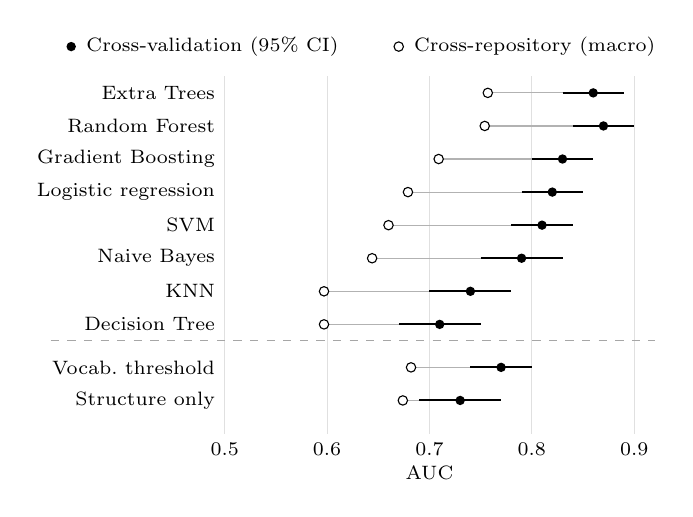
\begin{tikzpicture}[x=13cm, y=0.42cm, font=\scriptsize]
  % x coordinate = AUC - 0.5
  \foreach \t in {0.5,0.6,0.7,0.8,0.9} {
    \draw[black!12] ({\t-0.5},0.5) -- ({\t-0.5},-10.3);
    \node[below] at ({\t-0.5},-10.3) {\t};
  }
  \node at (0.2,-11.5) {AUC};
  \draw[dashed, black!35] (-0.17,-7.5) -- (0.42,-7.5);
  \foreach \y/\name/\cv/\ci/\lo in {
      0/Extra Trees/0.86/0.03/0.757,
      1/Random Forest/0.87/0.03/0.754,
      2/Gradient Boosting/0.83/0.03/0.709,
      3/Logistic regression/0.82/0.03/0.679,
      4/SVM/0.81/0.03/0.660,
      5/Naive Bayes/0.79/0.04/0.644,
      6/KNN/0.74/0.04/0.597,
      7/Decision Tree/0.71/0.04/0.597,
      8.3/Vocab.\ threshold/0.77/0.03/0.682,
      9.3/Structure only/0.73/0.04/0.674} {
    \node[left] at (0,-\y) {\name};
    \draw[black!30] ({\lo-0.5},-\y) -- ({\cv-0.5},-\y);
    \draw[line width=0.7pt] ({\cv-\ci-0.5},-\y) -- ({\cv+\ci-0.5},-\y);
    \fill ({\cv-0.5},-\y) circle (1.7pt);
    \draw[fill=white] ({\lo-0.5},-\y) circle (1.7pt);
  }
  \fill (-0.15,1.4) circle (1.7pt) node[right=2pt] {Cross-validation (95\% CI)};
  \draw[fill=white] (0.17,1.4) circle (1.7pt) node[right=2pt] {Cross-repository (macro)};
\end{tikzpicture}
\caption{AUC under cross-validation (filled, with 95\% CI; balanced folds) and macro AUC across repositories (hollow), by model and baseline. The axis starts at 0.5, the chance level.}
\label{fig:auc}
\end{figure}

\noindent\fbox{\parbox{\dimexpr\columnwidth-2\fboxsep-2\fboxrule\relax}{\textbf{RQ1.1 and RQ2:} vocabulary predicts flakiness in C\# well above chance (MCC 0.51--0.53, AUC 0.86--0.87 under cross-validation; AUC 0.75--0.78 across repositories), but its advantage is moderate: about $+$0.15 MCC over a structure-only model that already counts \texttt{await} expressions, only for the tree ensembles, and a ten-token rule matches the models on pooled AP across repositories. The practical value lies in ranking.}}

\subsection{RQ1.2: label robustness}
\label{sec:rq12}
The two rerun rounds diverge (Table~\ref{tab:sobreposicao}): of the 36 flaky units found by either of them, only 13 are flaky in both (Jaccard 0.36); 17 are flaky only in the 100-run round and 6 only in the 20-run round. The 20-run round finds 43\% of what the 100-run round finds, and the 100-run round finds 68\% of what the 20-run round finds. Part of this divergence is expected from the number of runs alone: a test that fails once in 100 runs has only about an 18\% chance of failing at least once in 20. Since a single flip on the same version shows that a test is flaky, all 36 units are flaky, and the divergence measures how many flaky tests each round misses rather than how many it gets wrong. \Den{Com a taxa de falha $p$ de cada teste na rodada de 100, somar $1-(1-p)^{20}$ para os 30 testes dá a sobreposição esperada, que pode ser comparada com os 13 observados (requer os dados de k/100). Treinar com o rótulo união (36) como análise adicional também requer execução.} Most tests exclusive to the 100-run round fail rarely (for example, Nerdbank.Streams 6$\to$0, NetMQ 2$\to$0), and of the six exclusive to the 20-run round, four are in NLog and three of them failed together in a single run, so they represent a single event. One of the tests exclusive to the 100-run round failed in all 20 controlled runs, which suggests an environmental difference between the rounds. \Den{Esse teste é \emph{broken} na rodada de 20, o que reforça que as rodadas diferem também no ambiente (SDK?), e não só no número de execuções. Investigar a causa (versão do SDK? dependência de data?) e reportar.} In LOPO with the 20-run labels, only five repositories have flaky tests, and the best macro AUC is 0.72. \Den{Este número não aparece em nenhuma tabela; incluir na Tab.~\ref{tab:cv100x20} ou no artefato.} With the 20-run labels (Table~\ref{tab:cv100x20}), the tree ensembles lose 0.07 to 0.14 MCC and 0.04 to 0.12 AUC, and the structure-only model (MCC 0.47) catches up with them within the confidence interval; the advantage of vocabulary holds only with the richer labels. \Den{A Tab.~\ref{tab:cv100x20} não mostra os ICs mencionados (``within the confidence interval''); incluí-los.}

\begin{table}[!h]
\caption{Overlap between the flaky units of the two rounds.}
\label{tab:sobreposicao}
\centering
\footnotesize
\begin{tabular}{@{}lcp{0.50\columnwidth}@{}}
\toprule
\textbf{Category} & \textbf{Units} & \textbf{Where} \tabularnewline
\midrule
Flaky in both & 13 & \raggedright StreamJsonRpc 5, MassTransit.Tests 3, Polly 2, Akka.NET 1, MassTransit.Abstractions 1, NLog 1 \tabularnewline[2pt]
Only in 100 runs & 17 & \raggedright Nerdbank.Streams 6, StreamJsonRpc 3, NetMQ 2, MassTransit.Tests 2, Testcontainers 1, Quartz 1, NLog 1, Polly 1 \tabularnewline[2pt]
Only in 20 runs & 6 & \raggedright NLog 4, MassTransit.Tests 1, Polly 1 \tabularnewline
\bottomrule
\end{tabular}
\end{table}

\begin{table}[!h]
\caption{Cross-validation with 100-run vs.\ 20-run labels (19 flaky units in the latter).}
\label{tab:cv100x20}
\centering
\footnotesize
\setlength{\tabcolsep}{5pt}
\begin{tabular}{@{}lcccc@{}}
\toprule
 & \multicolumn{2}{c}{\textbf{MCC}} & \multicolumn{2}{c}{\textbf{AUC}} \\
\cmidrule(lr){2-3}\cmidrule(lr){4-5}
\textbf{Model} & \textbf{100$\times$} & \textbf{20$\times$} & \textbf{100$\times$} & \textbf{20$\times$} \\
\midrule
Extra Trees       & 0.53 & 0.43 & 0.86 & 0.82 \\
Random Forest     & 0.51 & 0.44 & 0.87 & 0.80 \\
Gradient Boosting & 0.51 & 0.37 & 0.83 & 0.71 \\
\midrule
\multicolumn{5}{@{}l}{\emph{Baselines}} \\
Vocab.\ threshold & 0.40 & 0.23 & 0.77 & 0.66 \\
Structure only    & 0.36 & 0.47 & 0.73 & 0.77 \\
Random            & 0.02 & 0.04 & 0.53 & 0.54 \\
\bottomrule
\end{tabular}
\end{table}

As an independent check, the six tests flaky only in the 20-run round are labeled stable under the 100-run labels and receive a score when their own repository is held out, so the model has never seen them as positives. Three of them rank in the top 15\% of their repository (percentiles 0.96, 0.95, and 0.85), and the three NLog tests that failed together fall at percentiles 0.30--0.42. Counting the trio as a single event, three of four independent events are ranked high. With only four events, this check is anecdotal, but it points in the same direction as the cross-repository results.

\medskip
\noindent\fbox{\parbox{\dimexpr\columnwidth-2\fboxsep-2\fboxrule\relax}{\textbf{RQ1.2:} the lexical signal persists across rounds, but whether it beats structure depends on the round that produced the labels. The round changes which tests are flaky (Jaccard 0.36), largely because 20 runs miss rarely failing tests, and with the 20-run labels the structure-only model matches the ensembles.}}
\medskip

\subsection{RQ3: the vocabulary of flaky tests in C\#}
\label{sec:rq3}
Table~\ref{tab:tokens} shows the tokens with the highest information gain that occur in flaky tests from at least three repositories. The most informative markers are Task-based concurrency, that is, operations run in the background and awaited with \texttt{async}/\texttt{await} (\texttt{task} in 80\% of flaky tests vs.\ 31\% of stable ones; \texttt{async}/\texttt{await} in 67\% vs.\ 30\%), time handling (\texttt{TimeSpan}, \texttt{CancellationToken}, \texttt{Sleep}, \texttt{Delay}), and resource lifecycles (\texttt{Dispose}, \texttt{StopAsync}), along with rare, specific markers such as \texttt{GC} and \texttt{WeakReference} (Table~\ref{tab:marcadores}). This is consistent with the asynchronous-wait and concurrency causes reported for other languages \cite{luo2014empirical, barbosa2023test} and with the sleep/timeout pattern described for .NET \cite{leesatapornwongsa2022flakerepro}. The frequent markers are general: \texttt{task}, \texttt{async}, and \texttt{await} occur in six repositories. However, a third of stable tests in C\# also contain \texttt{async}/\texttt{await}, which explains why presence rules are weak. \Den{(i) Uma comparação sistemática com os vocabulários de Java, JS e Swift (ver o comentário da introdução sobre uma RQ cross-language) sustentaria a frase sobre consistência com outras linguagens, que suavizei. (ii) Os números ``80\% vs.\ 31\%'' e ``67\% vs.\ 30\%'' não estão na Tab.~\ref{tab:tokens}, que não tem a coluna \%S.}

\Den{Tab.~\ref{tab:tokens}: adicionar \%S, o número de repositórios e o lift (requer os dados; tirei o \%S da legenda porque a coluna não existe). Explicar tokens pouco intuitivos como \texttt{length}, \texttt{enumerable} e \texttt{writeline} (este pode refletir saída de log/diagnóstico, não uma causa). O filtro ``$\geq$3 repositórios'', aplicado depois de ver o ranking bruto, pode parecer \emph{cherry-picking}: mostrar o ranking bruto (no artefato ou numa coluna) e justificar o critério \emph{a priori}.}
\begin{table}[!h]
\caption{Top tokens by information gain (IG, in nats) present in flaky tests from at least three repositories. \%F: proportion of the 30 flaky units containing the token.}
\label{tab:tokens}
\centering
\footnotesize
\setlength{\tabcolsep}{12pt}
\begin{tabular}{@{}lrr@{}}
\toprule
\textbf{Token} & \textbf{IG} & \textbf{\%F} \\
\midrule
\texttt{task}              & 0.145 & 80 \\
\texttt{async task}        & 0.084 & 67 \\
\texttt{await}             & 0.084 & 67 \\
\texttt{async}             & 0.082 & 67 \\
\texttt{length}            & 0.065 & 27 \\
\texttt{await task}        & 0.061 & 23 \\
\texttt{server}            & 0.056 & 23 \\
\texttt{enumerable}        & 0.044 & 13 \\
\texttt{logger}            & 0.044 & 20 \\
\texttt{fromseconds}       & 0.043 & 20 \\
\texttt{writeline}         & 0.038 & 17 \\
\texttt{timespan}          & 0.034 & 23 \\
\texttt{dispose}           & 0.034 & 13 \\
\texttt{cancellationtoken} & 0.025 & 13 \\
\bottomrule
\end{tabular}
\end{table}

The raw information-gain ranking is dominated by project conventions: \texttt{trait}, \texttt{fact trait}, and \texttt{checkgcpressureasync} come only from StreamJsonRpc, and \texttt{trait} originates from an attribute, not from the test body. This dominance is itself evidence that part of what the models learn is the identity of the project (Section~\ref{sec:discussion}). Information gain favors frequent tokens; we therefore also report rare but specific markers by lift (Table~\ref{tab:marcadores}). They fall into memory and garbage collection (\texttt{gc}, \texttt{weakreference}), asynchronous composition (\texttt{whenall}), cancellation (\texttt{cancellationtokensource}), lifecycles (\texttt{stopasync}, \texttt{disposed}), and fixed waits (\texttt{sleep}, \texttt{task delay}). Each occurs in only two to four flaky tests, so they are exploratory. \Den{O IG leave-one-project-out (comentário no Step~6) quantificaria a dominância de StreamJsonRpc (requer execução).}

\Den{Tab.~\ref{tab:marcadores}: explicar os ``---'' (por que só alguns tokens foram testados?). O lift com 2 ocorrências é instável; considerar um IC ou suavização (lift com pseudo-contagem). Conferi que o menor $p$ (\texttt{gc}, $\approx 10^{-5}$) não sobrevive a Bonferroni ($\approx 10^{-6}$), e isso agora está na legenda.}
\begin{table}[!h]
\caption{Rare, specific markers (at least two flaky tests in at least two repositories, except \texttt{weakreference}). $p$-values: one-sided Fisher's exact tests; none survives a Bonferroni correction for the roughly 48,000 candidate tokens, so the table is exploratory.}
\label{tab:marcadores}
\centering
\scriptsize
\setlength{\tabcolsep}{5pt}
\begin{tabular}{@{}lrrrrr@{}}
\toprule
\textbf{Token} & \textbf{Flaky} & \textbf{\%F} & \textbf{\%S} & \textbf{\emph{Lift}} & \textbf{\emph{p}} \\
\midrule
\texttt{gc}                      & 3 & 10.0 & 0.12 & 84$\times$ & $<$0.001 \\
\texttt{weakreference}           & 2 &  6.7 & 0.18 & 37$\times$ & 0.002 \\
\texttt{stopasync}               & 2 &  6.7 & 0.12 & 56$\times$ & --- \\
\texttt{disposed}                & 2 &  6.7 & 0.13 & 50$\times$ & --- \\
\texttt{whenall}                 & 4 & 13.3 & 0.62 & 22$\times$ & --- \\
\texttt{cancellationtokensource} & 4 & 13.3 & 1.56 &  9$\times$ & --- \\
\texttt{sleep}                   & 2 &  6.7 & 0.82 &  8$\times$ & 0.03 \\
\texttt{task delay}              & 2 &  6.7 & 0.97 &  7$\times$ & 0.04 \\
\bottomrule
\end{tabular}
\end{table}

\myparagraph{Relation to root causes} The markers connect to the causes of flakiness described in the Introduction. \texttt{task}, \texttt{async}, and \texttt{await} indicate background operations whose completion the test must await, the territory of race conditions. \texttt{TimeSpan}, \texttt{FromSeconds}, \texttt{CancellationToken}, \texttt{Sleep}, and \texttt{Delay} indicate dependence on time and timeouts. \texttt{Dispose}, \texttt{StopAsync}, \texttt{server}, \texttt{logger}, and \texttt{WriteLine} indicate external resources that must be created and released, such as servers and output streams. \texttt{GC} and \texttt{WeakReference} indicate dependence on the garbage collector, whose timing is nondeterministic. This reading is an interpretation of the tokens, not a confirmed classification of each test's cause. \Den{Sugestão de alto impacto e baixo custo: com apenas 36 flaky, dá para rotular manualmente a causa raiz de cada um (taxonomia de Luo et al., dois avaliadores, kappa de Cohen) e cruzar categorias com tokens. Isso transforma a interpretação em evidência, responde à pergunta ``o vocabulário captura a causa?'' e é uma contribuição empírica nova para C\#.}

\myparagraph{Stability markers} Unlike Swift, where \texttt{xctassertequal} marks clearly synchronous tests, we found no robust stability marker: among the tokens present in flaky tests from at least three repositories, the only one more frequent in stable tests is \texttt{assert} (67\% vs.\ 69\%), which does not discriminate. The token \texttt{areequal} (0\% vs.\ 20\%) is an NUnit assertion style used by repositories without flaky tests, so it reflects the choice of framework, not stability. \Den{Conferir: a Seção~\ref{sec:subjects} diz que MassTransit e Quartz.NET usam NUnit e ambos têm flaky, então ``NUnit assertion style used by repositories without flaky tests'' não é exato (talvez eles usem \texttt{Assert.That}). De todo modo, o exemplo mostra que o modelo pode aprender framework/repositório, o que reforça a necessidade do baseline de repositório e da amostragem pareada.}

\medskip
\noindent\fbox{\parbox{\dimexpr\columnwidth-2\fboxsep-2\fboxrule\relax}{\textbf{RQ3:} flakiness in C\# is signaled by \texttt{Task}-based concurrency, time handling, and resource lifecycles, complemented by rare markers such as \texttt{GC} and \texttt{WeakReference}. The frequent markers are general across repositories, the rare ones are specific but backed by few tests, the raw ranking is dominated by the conventions of a single project, and no robust stability marker emerged.}}
\medskip

\subsection{RQ4: error analysis}
\label{sec:rq4}
To analyze errors, we use the LOPO scores, in which each test is scored by models trained without its repository. The score is the mean of Random Forest and Extra Trees over the 10 undersampling draws. In each of the nine repositories that have flaky tests, we rank all labeled tests (flaky and stable) by score, breaking ties by average rank, and compute each test's percentile within its repository, so that 1.0 corresponds to the highest-scoring test. The 30 flaky tests have a median percentile of 0.80; 9 have a percentile of at least 0.90, that is, they are in the top 10\% of their repository, 23 have a percentile of at least 0.75, in the top 25\%, and 6 fall below the median. This means that, if each repository were ranked by the model and the top quartile were selected for rerunning (about a quarter of the tests), that quartile would contain 77\% of the flaky tests, against about 25\% expected by chance, with a 95\% Clopper--Pearson confidence interval of 58\% to 90\%. \Den{\textbf{Falta o mais importante: comparar com os baselines na mesma métrica} (requer execução). Pela Seção~\ref{sec:rq3}, o token \texttt{task} sozinho está em 80\% dos flaky e em 31\% dos estáveis: rerodar só os testes com \texttt{task} cobre $\approx$80\% dos flaky com $\approx$31\% do esforço, quase o mesmo custo-benefício do modelo (77\% com 25\%). É preciso mostrar a curva recall vs.\ fração rerodada para o modelo, a regra, o estrutural, \texttt{task}/\texttt{async} e o aleatório. Se o modelo não ganhar com clareza da regra de um token, a recomendação de usar o ranking para priorizar reruns fica frágil.} The result also does not depend on the repositories that concentrate the positives: in the three largest (20 of the 30 flaky tests), 14 are in the top quartile (70\%), and in the other six repositories, 9 of 10 (90\%), although these have only one or two each.

This estimate should be read with caution. The two models that make up the score were chosen for their performance on the same data, and the confidence interval treats tests as independent, even though they come from a convenience sample and some are correlated (three NLog tests failed together), so the real uncertainty is probably larger. We also assume the same execution cost per test, which probably underestimates the real cost, since asynchronous tests and tests with fixed waits tend to be slower. Moreover, the result measures how concentrated flaky tests are at the top of the ranking, not the chance that rerunning reveals the flakiness, which depends on how often each test fails.

We also examined, in the test source code, the errors for the tests the model did not place in the top quartile (seven of the 30) and for the highest-scoring stable tests. \Den{Descrever o protocolo: quantos estáveis de maior score foram examinados (top-10 por repositório?), quem analisou (um ou dois autores?) e como as divergências foram resolvidas. Dos 7 falsos negativos, só 5 são discutidos.} This is a qualitative analysis of a few examples, not a count of causes. The false negatives are flaky tests whose cause lies beyond the reach of vocabulary. Three patterns recur. (i) The test merely delegates to a helper method: \texttt{JsonRpcPerf\_Pipe} and \texttt{JsonRpcPerf\_Channel} (Nerdbank.Streams) are one-line calls to a shared helper, with no assertions, so the cause lies outside the test body; \texttt{InvokeWithProgressParameter\_\allowbreak NoMemoryLeakConfirm} (StreamJsonRpc) awaits a helper, forces \texttt{GC.Collect()}, and checks a \texttt{WeakReference}, and its nondeterminism comes from garbage collection. (ii) Fixed waits without asynchronous constructs: \texttt{ReconnectOnRouterBug} (Section~\ref{sec:motivation}) synchronizes only through \texttt{Thread.Sleep}, a token present in only two flaky tests and weakly learned. (iii) Time and global state: MassTransit's \texttt{Should\_be\_using\_the\_\allowbreak correct\_algorithm\_\allowbreak for\_sequential\_guids} installs a tick provider and compares parts of consecutively generated identifiers, which depends on the clock and, apparently, on shared static state.

The false positives are stable tests that use concurrency and time deterministically. Polly's \texttt{Execute\_CallerCancellation\_\allowbreak EnsureExceptionCarriesCallerToken} uses an injected time provider and a cancellation token, being asynchronous and time-related, yet deterministic by construction; Quartz's \texttt{Trigger\_Fires\_After\_Clock\_\allowbreak Jumps\_Backward\_And\_Returns} controls time through a custom provider and awaits a \texttt{TaskCompletionSource} instead of sleeping. The model detects the constructs but does not judge whether they are used well. Akka.NET's \texttt{A\_CircuitBreaker\_stress\_test} uses a fixed \texttt{await Task.Delay(3000)} with a wide margin and may be latently flaky beyond our 120 runs, so some false positives may be label noise. \Den{Experimento barato e convincente: rerodar os $\sim$20 falsos positivos de maior score de 500 a 1.000 vezes e/ou sob stress de CPU. Se alguns falharem, há evidência de que o modelo encontra flaky latentes (e de que os rótulos por rerun subestimam a flakiness), o que vira um resultado positivo forte.}

\medskip
\noindent\fbox{\parbox{\dimexpr\columnwidth-2\fboxsep-2\fboxrule\relax}{\textbf{RQ4:} the model fails when the cause is hidden in helper methods, in GC behavior, or in shared state (false negatives), and when asynchronous or time constructs are used with controlled time or event-based synchronization (false positives). Judging whether usage is correct requires semantic, not lexical, analysis.}}
\medskip

\subsection{Sensitivity analyses}
\label{sec:sensitivity}
We tested two threats to the vocabulary signal, keeping the labels, undersampling seeds, and folds fixed so that the comparison is paired. \Den{Se a comparação é pareada, aplicar um teste pareado (Wilcoxon sobre as 50 estimativas) e reportar $p$ e tamanho de efeito.} Without attributes: we removed all tokens inside attribute lists (\texttt{[Fact]}, \texttt{[Trait(...)]}, \texttt{[InlineData(...)]}), so that project conventions do not drive the prediction. With helpers: we added to each test the tokens of the helper methods it calls, resolved by name (at most five helpers per test, one level only); the expansion resolved at least one helper in 67\% of the methods, and, since resolution is by name, without type information, some helpers may merely share a name with the one actually called. \Den{O artigo já usa Roslyn: com o \texttt{SemanticModel}, resolver as chamadas com informação de tipo é direto e elimina a ambiguidade por nome. Como os helpers são o principal padrão de falso negativo (RQ4), essa melhoria tem ótimo custo-benefício e pode virar uma contribuição técnica.}

\begin{table}[!h]
\caption{Sensitivity of cross-validation MCC and LOPO macro AUC (original features, without attributes, with one-level helpers).}
\label{tab:sensibilidade}
\centering
\scriptsize
\setlength{\tabcolsep}{3.5pt}
\begin{tabular}{@{}lcccccc@{}}
\toprule
 & \multicolumn{3}{c}{\textbf{MCC (CV)}} & \multicolumn{3}{c}{\textbf{Macro AUC (LOPO)}} \\
\cmidrule(lr){2-4}\cmidrule(lr){5-7}
\textbf{Model} & \textbf{orig.} & \textbf{no attr.} & \textbf{+help.} & \textbf{orig.} & \textbf{no attr.} & \textbf{+help.} \\
\midrule
Extra Trees         & 0.53 & 0.46 & 0.56 & 0.757 & 0.737 & 0.764 \\
Random Forest       & 0.51 & 0.46 & 0.53 & 0.754 & 0.721 & 0.773 \\
Gradient Boosting   & 0.51 & 0.49 & 0.43 & 0.709 & 0.683 & 0.643 \\
Logistic regression & 0.44 & 0.43 & 0.49 & 0.679 & 0.673 & 0.714 \\
\midrule
\multicolumn{7}{@{}l}{\emph{Baseline}} \\
Structure only      & 0.36 & 0.36 & 0.36 & 0.674 & 0.674 & 0.674 \\
\bottomrule
\end{tabular}
\end{table}

Removing attributes reduces the MCC of the two best ensembles from 0.53 to 0.46 (Extra Trees) and from 0.51 to 0.46 (Random Forest), but keeps AUC at 0.84--0.85: \Den{Esses valores de AUC não estão na Tab.~\ref{tab:sensibilidade} (que mostra MCC da CV e AUC do LOPO). Incluir a coluna ou remover.} attributes carry part of the signal, plausibly project conventions, but most of it lies in the test body, and the ensembles remain well above the structure-only baseline. Adding helpers slightly improves the ensembles (MCC 0.56 and 0.53) and improves the linear and probabilistic models more, but hurts Gradient Boosting (from 0.51 to 0.43) and the Decision Tree (from 0.44 to 0.39). \Den{O Decision Tree não está na Tab.~\ref{tab:sensibilidade}. Incluir ou remover.} The ensembles' gains are within the confidence intervals. The naive one-level expansion therefore does not eliminate the helper blind spot: it adds tokens to two thirds of the tests, flaky or stable alike.


\section{Discussion}
\label{sec:discussion}

\myparagraph{Practical use} What the model does well is order tests, not decide whether each one is flaky. When it flags a test as flaky, it is right only 2 or 3 times out of 100, so using it to block a delivery in the pipeline would raise too many false alarms. Its usefulness appears when we consider a team that lacks the time to rerun every test and must choose where to start. In that case, the ranking works as a priority list: the top quarter of each project's list concentrates 77\% of the flaky tests (Section~\ref{sec:rq4}), and rerunning that quarter would cost about a quarter of the total effort, if each test took roughly the same time. An example helps show the gain: in a repository of 1,000 tests at the natural rate of 0.39\%, there are about 4 flaky tests; the top quartile has 250 tests and, with 77\% coverage, about 3 of them, a density of roughly 1.2\%, three times that of the whole set, though still low for gating. \Den{Um lift de 3$\times$ é modesto e precisa ser comparado com a heurística trivial ``rerodar só os testes com \texttt{task}/\texttt{async}'' (ver o comentário na RQ4; requer execução). Se a heurística der o mesmo ganho, a recomendação prática deveria ser ela, e o modelo fica dispensável. Isso precisa ser enfrentado explicitamente.} This holds as long as rerunning actually reveals the flakiness, which depends on how often each test fails. There is also a secondary benefit: the vocabulary analysis shows which constructs tend to accompany flakiness, such as fixed waits (\texttt{Sleep}), cancellation, and garbage collection, and a code reviewer can use these cues as warnings during review. We did not test this use with practitioners. The ranking can also select which tests to hand to dynamic tools that reproduce concurrency failures, such as FlakeRepro \cite{leesatapornwongsa2022flakerepro}, which need the test and an observed failure to work.

\myparagraph{Part of the signal is project-specific} When the model is trained and tested on tests from all projects mixed together, it performs very well (AUC of 0.86--0.87). When it must predict the tests of a project it has never seen, performance drops (AUC of 0.75--0.78). This drop indicates that part of what the model learns is each project's writing habits, not flakiness itself. Three repositories hold two thirds of the flaky tests (20 of 30), removing attributes reduces MCC by about 0.05 to 0.07, and the tokens with the highest information gain come largely from a single project. On the other hand, cross-repository performance remains well above chance, which shows that a general signal also exists. In practice, this calls for caution when importing results from other teams and languages, and, if the tool is adopted in an organization, it is worth calibrating it with the flaky tests that organization already knows about. \Den{Esta é a discussão central do paper de Go (``what classifiers actually learn''). Para manter a coerência entre os trabalhos do grupo, e porque o revisor pode ser o mesmo, adotar aqui os mesmos diagnósticos: baseline só com o nome do repositório e IG leave-one-project-out (requer execução). Sem eles, ``part of the signal is project-specific'' fica só qualitativo.}

\myparagraph{Comparison with other ecosystems} In Swift, the same kind of classifier reached an MCC of 0.75 under balanced cross-validation, against 0.08 for the best baseline \cite{medeiros2026vocabulary}; in C\#, the MCC is 0.51--0.53, and the non-trivial baselines reach 0.36--0.40. The precision, recall, and F1 of our best model are also lower than those reported for Java, Python, JavaScript, and Swift (Table~\ref{tab:literatura}). The numbers are not directly comparable, because the datasets, labels, protocols, and number of positives differ (91 flaky in Swift, 30 here), but they suggest that the flakiness vocabulary in C\# is less distinctive: asynchronous constructs are also common in stable tests, and there is no stability marker like Swift's \texttt{xctassertequal}.

\myparagraph{Toward better features} The errors point to natural extensions: propagating tokens through the helper methods called (interprocedural analysis) and designing features that separate fixed waits from controlled time. A simple version of the first, which adds to each test the tokens of the helpers it calls, brought small and inconsistent gains (Section~\ref{sec:sensitivity}); a proper analysis, with type information, is left for future work. The second requires distinguishing, in the code, a \texttt{Sleep} that assumes a duration from a \texttt{Delay} controlled by a simulated clock, which vocabulary alone cannot do.

\myparagraph{Methodological lessons} First, the unit of analysis changes the answer. A single test method can generate several cases that the runner reports separately: counting cases, there are 50 flaky tests; counting the methods that declare them, there are 30. In StreamJsonRpc, for example, the same test runs with six serializers and generates 25 flaky cases from only 8 methods. Second, labels depend on the round of runs: of the 36 flaky units found by either of the two rounds, only 13 are flaky in both, and the comparison between vocabulary and structure changes with the round (Section~\ref{sec:rq12}), so studies with a single round should report this sensitivity. Third, we document .NET-specific pitfalls that distorted our initial counts (Table~\ref{tab:armadilhas}): parameterized test names containing timestamps, thread ids, or dates, which make the same test look like several; differences between target frameworks; tests declared in base classes and executed in several derived classes; and contaminated environments, which produced spurious flaky tests.

\myparagraph{Recommendations for rerun studies in .NET} The pitfalls we encountered suggest a minimal protocol for anyone wishing to repeat this kind of study: (i) identify each test by its fully qualified class plus its display name and normalize timestamps, thread ids, and dates in the names; (ii) resolve inherited and parameterized tests to the declaring method and report both counts, per case and per method; (iii) build once, then run without rebuilding and on the same target framework in every round; (iv) isolate the environment between runs and discard contaminated rounds; and (v) report the sensitivity of the labels to the number of runs. \Den{Estas lições e este protocolo talvez sejam a contribuição mais original e reutilizável do artigo. Considerar uma seção própria (ou uma RQ), com o script de normalização/resolução de herança no artefato, como ferramenta. Seria ótimo quantificar quanto cada armadilha distorceria as contagens se não fosse tratada (ex.: quantos flaky espúrios surgem sem a normalização de nomes).}


\section{Threats to Validity}
\label{sec:threats}

\myparagraph{Construct validity} The labels come only from reruns, so tests whose flakiness does not reproduce on our machine are labeled stable, and the number of runs matters: fewer runs miss rarely failing tests, and the 20-run round identified only 13 of the 30 flaky tests identified with 100 runs. Test order was not randomized across runs, so order-dependent flakiness is likely underrepresented and our results concern mainly non-order-dependent flakiness. \Den{Confirmar que a ordem dos testes foi a mesma em todas as execuções e informar a configuração de paralelismo.} Environmental disruptions can also create spurious flaky tests; we mitigated them by discarding contaminated rounds and repeating them in isolation. The two rounds also differ in more than the number of runs: the .NET SDK used in the 100-run round was not recorded and may differ from the one resolved in the 20-run round, and Testcontainers was run only 5 times in the second round. Test identity is reconstructed from display names and class hierarchies, and a small number of tests could not be resolved to source code (none of them flaky in the 100-run round).

\myparagraph{Internal validity} The 1:1 undersampling balances the test folds and makes precision and F1 optimistic (LOPO quantifies the difference); correlated tests (for example, three NLog tests that failed together) may inflate the positive class; and the two best models were chosen on the same data on which they are evaluated. Attribute tokens may encode project conventions, and removing them reduces the MCC of the best models by about 0.05--0.07. Tokenization choices, such as which keywords are discarded and whether identifiers are split, affect the vocabulary, and the classifiers were not tuned. The qualitative error analysis was performed by the authors on a few examples and is subject to interpretation bias.

\myparagraph{Conclusion validity} The same 30 positives appear in every draw, so the confidence intervals underestimate uncertainty and, with so few positives, the ordering among classifiers is not reliable. The $p$-values of Table~\ref{tab:marcadores} do not survive a correction for the roughly 48,000 candidate tokens, and the rare markers are exploratory.

\myparagraph{External validity} Project selection was not random: it favored open-source libraries with unit tests and domains in which concurrency is common, and it excluded two projects whose suites depend on external servers, which underrepresents network-related flakiness. None of the projects uses MSTest. The 0.24\% rate and the results may therefore not generalize to applications, UI tests, or proprietary code; moreover, flakiness is concentrated in nine repositories, and the results are specific to the .NET toolchain and to the single Windows machine used, without additional load.


\section{Conclusion}
\label{sec:conclusion}
This work evaluated static prediction of flaky tests in C\# from code vocabulary. The lexical signal exists, but it is modest. Across the 17 projects, which total 19,211 executed test cases, corresponding to 12,665 labeled test methods, of which 30 are flaky, the best models reach an MCC of 0.51--0.53 and an AUC of 0.86--0.87 under cross-validation, only moderately above a structure-only model and a ten-token rule, and an AUC of 0.75--0.78 when the repository is unseen, with a precision of 2--3\% at the natural base rate. The signal rests on Task-based concurrency, time handling, and resource lifecycles. It fails when the cause of flakiness lies outside the test body, in a helper method, in garbage collector behavior, or in state shared between tests, and when stable tests use time and concurrency in a controlled way.

For practitioners, vocabulary is useful for prioritizing reruns, not for gating pipelines: the top quartile of each repository's ranking contains 23 of the 30 flaky tests. For researchers, the labels, and even the comparison between vocabulary and structure, depend on the rerun round, so rerun studies should resolve tests to their declaring methods, report the sensitivity of their labels, and follow the protocol of Section~\ref{sec:discussion}. As next steps, we plan to make the model follow calls between methods, so that it also reads the code of the helper methods the test uses; to design features that distinguish a fixed wait from time controlled by the test itself; to repeat the study with more projects, chosen at random; \Den{O revisor vai ler isso como ``por que não fizeram agora?''. Os 30 positivos são a principal fraqueza do artigo; se houver tempo antes do ISSTA, ampliar o dataset (mais projetos, rodada em CI/Linux, testes marcados pelos desenvolvedores) é a melhoria de maior retorno.} and to ask practitioners how they would use a test ranking to decide what to rerun.


% Required by the MSR 2027 Open Science Policy.
\section*{Data Availability}
The scripts used to execute the test suites and collect the reruns, the
resulting dataset of flaky and stable test methods, the feature extraction
and classification pipeline, and instructions to reproduce all results are
available in an anonymized replication package:\Fix{link}. \Den{Link placeholder: criar o repositório anônimo antes da submissão. Incluir no pacote: SHAs dos commits, lista de candidatos, TRX brutos, scripts de normalização de nomes (Tab.~\ref{tab:armadilhas}) e o ranking bruto de tokens.}

\bibliography{biblio}
\bibliographystyle{IEEEtran}

\end{document}